%%%%%%%%%%%%%%%%%%%%%%%%%%%%%%%%%%%%%%%%%
% Thesis 
% LaTeX Template
% Version 1.3 (21/12/12)
%
% This template has been downloaded from:
% http://www.latextemplates.com
%
% Original authors:
% Steven Gunn 
% http://users.ecs.soton.ac.uk/srg/softwaretools/document/templates/
% and
% Sunil Patel
% http://www.sunilpatel.co.uk/thesis-template/
%
% License:
% CC BY-NC-SA 3.0 (http://creativecommons.org/licenses/by-nc-sa/3.0/)
%
% Note:
% Make sure to edit document variables in the Thesis.cls file
%
%%%%%%%%%%%%%%%%%%%%%%%%%%%%%%%%%%%%%%%%%

%----------------------------------------------------------------------------------------
%	PACKAGES AND OTHER DOCUMENT CONFIGURATIONS
%----------------------------------------------------------------------------------------

\documentclass[11pt, a4paper, oneside]{Thesis} % Paper size, default font size and one-sided paper

\graphicspath{{./Pictures/}} % Specifies the directory where pictures are stored

\usepackage[square, numbers, comma, sort&compress]{natbib} % Use the natbib reference package - read up on this to edit the reference style; if you want text (e.g. Smith et al., 2012) for the in-text references (instead of numbers), remove 'numbers' 
\hypersetup{urlcolor=blue, colorlinks=true} % Colors hyperlinks in blue - change to black if annoying
\title{\ttitle} % Defines the thesis title - don't touch this

\begin{document}

\frontmatter % Use roman page numbering style (i, ii, iii, iv...) for the pre-content pages

\setstretch{1.3} % Line spacing of 1.3

% Define the page headers using the FancyHdr package and set up for one-sided printing
\fancyhead{} % Clears all page headers and footers
\rhead{\thepage} % Sets the right side header to show the page number
\lhead{} % Clears the left side page header

\pagestyle{fancy} % Finally, use the "fancy" page style to implement the FancyHdr headers

\newcommand{\HRule}{\rule{\linewidth}{0.5mm}} % New command to make the lines in the title page

% PDF meta-data
\hypersetup{pdftitle={\ttitle}}
\hypersetup{pdfsubject=\subjectname}
\hypersetup{pdfauthor=\authornames}
\hypersetup{pdfkeywords=\keywordnames}

%----------------------------------------------------------------------------------------
%	TITLE PAGE
%----------------------------------------------------------------------------------------

\begin{titlepage}
\begin{center}


\includegraphics[width=13cm]{Figures/Uni}\\[1.5cm] % University name
\textsc{\Large Master Thesis}\\[0.5cm] % Thesis type

\HRule \\[0.4cm] % Horizontal line
{\huge \bfseries Using models@runtime to build deployment and provisioning plans of multi-cloud applications}\\[0.4cm] % Thesis title
\HRule \\[1.5cm] % Horizontal line
 
\begin{minipage}[t]{0.4\textwidth}
\begin{flushleft} \large
\emph{Author:}\\
\href{https://no.linkedin.com/pub/maksym-lushpenko/28/a78/354}{Maksym Lushpenko} % Author name - remove the \href bracket to remove the link
\end{flushleft}
\end{minipage}
\begin{minipage}[t]{0.4\textwidth}
\begin{flushright} \large
\emph{Supervisors:} \\
\href{http://users.ics.forth.gr/~magoutis/}{Prof. Kostas Magoutis} \\ % Supervisor name - remove the \href bracket to remove the link 
\href{http://ferrynico.com/}{Dr. Nicolas Ferry} 
\end{flushright}
\end{minipage}\\[5cm]
 

\includegraphics[width=11cm]{Figures/Sintef}\\[1cm]
 
{\large \today}\\[4cm] % Date

 
\vfill
\end{center} 

\end{titlepage}


%----------------------------------------------------------------------------------------
%	ABSTRACT PAGE
%----------------------------------------------------------------------------------------

\addtotoc{Abstract} % Add the "Abstract" page entry to the Contents

\abstract{\addtocontents{toc}{\vspace{1em}} % Add a gap in the Contents, for aesthetics

Existing frameworks for the provisioning and deployment of multi-cloud applications usually rely on declarative (using application topology models) or imperative (using deployment plans) deployment approaches. Declarative approaches are considered to be easy to use, but not very flexible because the deployment logic is predefined, and users can not change it according to their needs. Imperative approaches allow explicit definition of every deployment action but are considered to be hard to write and maintain. Besides, imperative approaches usually rely on generic workflow definition languages to describe deployment plans. These languages are often too powerful and complex to be used in the deployment domain.

In this work, we combine both approaches by generating deployment plans from the application topology models and introduce a domain-specific language for the plans definition and manipulation. This allows application owners to deploy applications without much effort while having the ability to tune generated plans according to their needs. Moreover, we developed a deployment engine that shows the deployment process in real time. It helps developers to analyze, optimize and debug the deployment process.  

Finally, most applications have to be updated many times during their life-cycle. To do this efficiently (without redeploying the whole application or writing additional deployment plans) we exploit the models@runtime approach in combination with the plan generation mechanism. This combination reduces the complexity of the application updates and application delivery times by enabling seamless reconfigurations at run time, that only impact parts of the system that are going to be changed.    


}

\clearpage % Start a new page

%----------------------------------------------------------------------------------------
%	ACKNOWLEDGEMENTS
%----------------------------------------------------------------------------------------

\setstretch{1.3} % Reset the line-spacing to 1.3 for body text (if it has changed)

\acknowledgements{\addtocontents{toc}{\vspace{1em}} % Add a gap in the Contents, for aesthetics

\noindent The research leading to these results has received funding from the European Community's Seventh Framework Programme (FP7/2007-2013) under grant agreement number: 318484 (MODAClouds).

\noindent In addition, I am very grateful to Dr. Nicolas Ferry for the every day support and lengthy discussions of different thesis issues; to Prof. Kostas Magoutis, Dr. Arnor Solberg and Dr. Franck Chauvel for valuable comments on how to improve my thesis; to my friend Nikolay Nikolov for sharing his experience and helping me with the thesis preparation, and to the whole MDE research group at SINTEF.
}
\clearpage % Start a new page

%----------------------------------------------------------------------------------------
%	LIST OF CONTENTS/FIGURES/TABLES PAGES
%----------------------------------------------------------------------------------------

\pagestyle{fancy} % The page style headers have been "empty" all this time, now use the "fancy" headers as defined before to bring them back

\lhead{\emph{Contents}} % Set the left side page header to "Contents"
\tableofcontents % Write out the Table of Contents

\lhead{\emph{List of Figures}} % Set the left side page header to "List of Figures"
\listoffigures % Write out the List of Figures

\lhead{\emph{List of Tables}} % Set the left side page header to "List of Tables"
\listoftables % Write out the List of Tables


%----------------------------------------------------------------------------------------
%	THESIS CONTENT - CHAPTERS
%----------------------------------------------------------------------------------------

\mainmatter % Begin numeric (1,2,3...) page numbering

\pagestyle{fancy} % Return the page headers back to the "fancy" style

% Include the chapters of the thesis as separate files from the Chapters folder
% Uncomment the lines as you write the chapters

% Chapter 1

\chapter{Introduction} % Main chapter title

\label{Chapter1} % For referencing the chapter elsewhere, use \ref{Chapter1} 

\lhead{Chapter 1. \emph{Introduction}} % This is for the header on each page - perhaps a shortened title

%----------------------------------------------------------------------------------------

\noindent Cloud-based applications are typically large-scale systems that rely on complex software stacks. Managing such applications is not a trivial task, especially if the application spans across multiple cloud providers and different locations \cite{elmroth2011self}. Some of the important challenges during their lifecycle are (i) how to provision and deploy an application and (ii) how to manage its state and evolution. 

There are two main approaches to the resource provisioning and deployment of cloud applications: imperative and declarative. In this work we identify benefits and limitations of each approach with help of the motivating example, and show how a combination of both approaches can benefit application operators. In addition, to make the deployment process as simple as possible, we introduce a domain-specific language for the specification and manipulation of the deployment plans (a set of instructions on how to deploy an application). Using this language we can illustrate the deployment process in real-time, which helps application operators to analyze and optimize the process itself.  

Regarding the application state and evolution, a  common approache is to redeploy the whole application whenever it needs to be updated, another one is to write new updating scripts and execute them each time the running system should be updated. Such solutions are either cumbersome (because application operators have to maintain the list of scripts) or not efficient (because cloud resources must be deprovisioned for the old system and provisioned again for the new one). In this work we show how the usage of the models@runtime pattern in combination with our domain-specific language allows to update applications efficiently and without much effort.

Finally, we conduct a set of deployment experiments to validate and evaluate the proposed solutions.

The results of this thesis are included in the paper to be submitted in the models@runtime workshop at the ACM/IEEE MODELS 2015 conference\footnote{ ACM/IEEE MODELS 2015 conference, http://www.modelsconference.org/}.


%----------------------------------------------------------------------------------------

\section{Research Motivation}

In this section we outline several reasons how the research presented in this paper  addresses important concerns of the cloud application operators.

\subsection{Background}

\noindent As we mentioned earlier, important challenges during the life-cycle of cloud applications include (i) how to provision and deploy an application and (ii) how to manage its state and evolution. 

\noindent Provisioning\footnote{ OGSA Glossary of Terms v.1.6, $  $https://redmine.ogf.org/dmsf\_files/10963?download=} of the application means allocation of the required resources on the chosen cloud. Resources may be virtual machines, storage, load balancers, domain name system (DNS) records and more. Every cloud provider exposes a self-service portal and an Application-Programming Interface (API) that can be exploited to provision cloud resources, but most of those interfaces have different syntax and behavior thus introducing a so-called vendor lock-in. As a result, cloud application providers planning to run different components of their application on different clouds (e.g., a database on Amazon and a web server on Google) have to manage different APIs. This issue has been partially solved by libraries such as jclouds\footnote{ Apache jclouds, $  $http://jclouds.apache.org/} or deltacloud\footnote{ Deltacloud, https://deltacloud.apache.org/ }, which provide a uniform interface to access all major cloud providers. For instance, in jclouds, operators can define minimum RAM and CPU requirements for their virtual machines and it will try to allocate them on the chosen cloud according to cloud provider's capabilities. Nevertheless, when cloud application providers are not limiting themselves to the infrastructure level and want to provision particular application components on Platform-as-a-Service (PaaS),  they have to rely on diverse cloud provider-specific APIs. To handle this heterogeneity a standardization effort has been made which led to the specification of the Cloud Application Management for Platforms (CAMP) standard \cite{CAMP-v1.1}. Still, the challenge remains to provision Infrastructure-as-a-Service (IaaS) and PaaS level application components at the same time.

\noindent 

\noindent Deployment refers to all activities required to make the cloud application ready for use \cite{specification2006deployment}. Deployment activities encompass tasks such as downloading and installing all required software components, configuring them and establishing connections with other relevant components (e.g., connect caching server to the web server). Challenging aspects of the deployment phase are how to ensure the proper order of installation between different components and how to share relevant data between them (e.g., how to configure database URL in the web server if the database is located on the different virtual machine and internet protocol (IP) address of that machine is not known in advance).

\noindent 

\noindent The provisioning and deployment tasks may be done manually or automatically. Manual execution of these tasks is not suitable for large-scale cloud applications because it is error-prone, not time-efficient and hardly feasible if many virtual machines and software packages have to be installed and configured. Therefore, application developers and operators are looking for automation. Automation of these tasks typically has two flavors: declarative and imperative \cite{INPROC-2013-45}. The imperative approach requires the explicit definition of how to reach the desired state of the application in the application deployment plan, usually by means of some general workflow language. The deployment plan is a workflow - a set of atomic tasks that are executed in a specific order (some of them may run in parallel). The imperative approach gives developers full control over the deployment process but reduces the reusability of the solution because writing in the first place and then changing such plans is not a trivial task. In contrast, the declarative approach requires only specification of the desired final state of the application. This state is usually described in the application topology model or blueprint using a domain-specific language (DSL), and then exact steps on how to reach that state will be derived from this model by the deployment engine. Such an approach allows developers to reuse their topology model in different scenarios by doing small updates to the model. Nevertheless, the generation of the deployment plan relies on a set of predefined rules, and since  these rules are typically not subject to change, all possible plans can not be generated. In addition, generated plans may not be optimal because they were generated according to the default rules. ~We will illustrate each approach and their limitations in the motivating example. 

\noindent 

\noindent Application management after the deployment (runtime phase) includes monitoring, error handling, software updates, dynamic reconfiguration and scaling operations. Among the challenging tasks is the dynamic reconfiguration of the system, which may include evaluation of dependencies between system components and their current state, calculation of the required changes to the application, generation of the adaptation plan, and its execution \cite{arshad2007deployment}. Dynamic reconfiguration includes scaling of the application, which may be achieved by moving the application to a more powerful server (scale-up) or by deploying it to multiple interconnected servers, possibly with a load balancer (scale-out) \cite{michael2007scale}. Manually, it could be done by updating the application topology model for instance via API calls to some application manager or via command-line tools if there are any. In automatic way, scalability may be achieved with help of policies that define when the application or some part of it shall be scaled in or out (or up or down), this exploits one of the main features of the clouds called elasticity: ``Elasticity is the degree to which a system is able to adapt to workload changes by provisioning and deprovisioning resources in an autonomic manner, such that at each point in time the available resources match the current demand as closely as possible'' \cite{herbst2013elasticity}. 

\noindent 

\noindent The complexity of specifying application deployment (either via application topology model or deployment plan) and of maintaining and thus dynamically adapting the deployment of cloud application are important challenges faced by cloud application operators. The proposed approach tackles these challenges by enabling the automatic plan generation, based on a declarative specification of the target application topology, and the specification of detailed deployment plans, based on an imperative approach, together with support for the dynamic reconfiguration of the running system in an efficient and controllable manner by exploiting models@runtime technologies.

\noindent 

\noindent In the motivating example we aim to showcase the pros and cons of different deployment approaches and difficulties of management tasks such as dynamic reconfigurations of the deployment of a cloud-based applications. This will provide us with a basis to formulate our research goal.

%----------------------------------------------------------------------------------------

\subsection{Motivating Scenario}

\noindent To have a better understanding of the previously discussed challenges and approaches, the following motivating scenario has been developed: installation of a distributed real-time computation system called Apache Storm\footnote{ Apache Storm, $  $https://storm.apache.org/}. The architecture of the Apache Storm is shown on Figure \ref{fig:Storm}. and in short consists of a master node (nimbus), which assigns tasks to slave nodes (supervisors) whilst all coordination between master and slave nodes is done with help of the Zookeeper\footnote{ Apache Zookeeper, $  $https://zookeeper.apache.org/} cluster (a service which enables reliable distributed coordination). 

\noindent 

\begin{figure}[htbp]
	\centering
		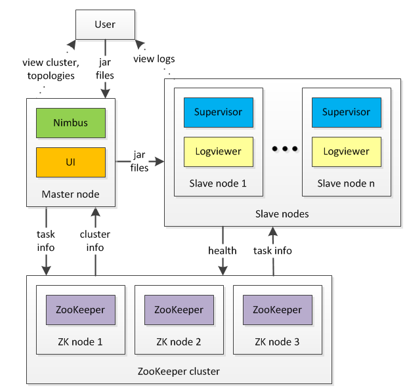
\includegraphics{./Figures/Storm_architecture}
		\rule{38em}{0.5pt}
	\caption[Storm Architecture]{Apache Storm architecture (http://jansipke.nl/storm-in-pictures/)}
	\label{fig:Storm}
\end{figure}

\noindent

\noindent \textbf{\textit{System setup}}. For our scenario, we consider one master node, one zookeeper node, and three slave nodes. Each node is a virtual machine running Ubuntu 14.04 as operating system, the master and slave nodes will be hosted on Amazon EC2\footnote{ AWS Command Line Interface, $  $http://docs.aws.amazon.com/cli/latest/userguide/cli-chap-welcome.html} and zookeeper node on OpenStack\footnote{ OpenStack Command Line Interface, $  $http://docs.openstack.org/cli-reference/content/}. Even for such a simple system, manual provisioning of virtual machines and installation of software components could take from a few hours to one day, assuming the user already knows how to install everything and in which order. In addition, application deployment must be reproducible, which is hardly the case for the manual approach. That is why we need some sort of automation: declarative or imperative. In addition, we will detail the challenges that arise after the application deployment.  

\noindent

\noindent \textbf{\textit{Imperative approach}}. Both Amazon EC2 and OpenStack have a command-line interface (CLI) which can be used for provisioning of virtual machines (APIs could also be used, but for simplicity we went for CLI). So, assuming the command line tools are installed, we could create a bash script or a deployment plan similar to the pseudocode\footnote{ Pseudocode standard, $  $http://users.csc.calpoly.edu/\~{}jdalbey/SWE/pdl\_std.html} depicted in Listing \ref{lst:1}.

\noindent Such plan would automate the whole process of provisioning and deployment of storm cluster on Amazon and OpenStack infrastructures. If we wrap-up part of the code in black font into ``init'' function and the one in blue font into ``add\_slave'' function, we would create management operations which could be used through the life-cycle of our application.

\begin{center}
	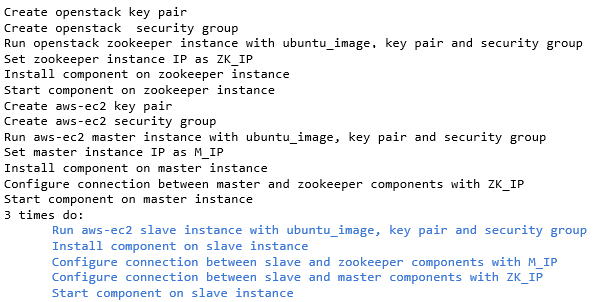
\includegraphics[width=38em]{./Figures/Imperative}
	\begin{lstlisting}[mathescape,caption={Imperative approach to deploy storm cluster},label={lst:1}]
	\end{lstlisting}
\end{center}

\noindent However, what if we would like to run the zookeeper server on Amazon? We would have to rewrite part of the provisioning and deployment plan. Moreover, in the situation when one zookeeper node can not cope with the imposed workload, there is a need to change to a cluster of zookeeper nodes. In that case we would have to change the whole plan because then the master node and every slave node needs to know IP addresses of all zookeeper nodes (also all zookeeper nodes have to know about each other), so the number of connections would grow exponentially. 

\noindent


\noindent Rising these questions shows us that imperative automation approaches handle well provisioning and deployment tasks because developers have fine-grained control of every step in the deployment plan, but they are less reusable and usually tied to one specific scenario.

\noindent 

\noindent \textbf{\textit{Declarative approach}}. As mentioned before, in declarative approaches application operators need to define the structure of the application and then the deployment plan will be derived from that structure and executed in the proper order by the deployment engine. The deployment engine will also take care of the data exchange between different tasks like an exchange of IP addresses of virtual machines. We used CloudML \cite{FerrySongRCS14} as an example of such approach. There we had to describe our desired providers, virtual machines, software components and relations between them. A folded representation of the JSON description of the storm CloudML application topology model from the JSON online editor\footnote{ JSON online editor, https://www.jsoneditoronline.org/} is shown on Figure \ref{fig:JSON}:

\noindent

\begin{figure}[htbp]
	\centering
		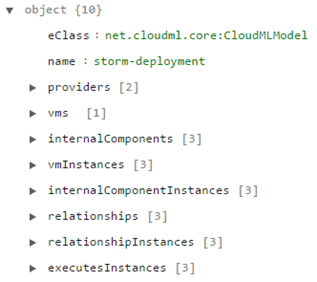
\includegraphics{./Figures/Declarative}
		\rule{38em}{0.5pt}
	\caption[Declarative Approach]{CloudML application model in JSON}
	\label{fig:JSON}
\end{figure}

\noindent

\noindent Providers, vms, internalComponents and relationships sections define reusable types, while other sections - instances of these specific types. The order of provisioning and deployment is based on components' requirements. For instance, zookeeper internal component type requires an Ubuntu based platform as illustrated in Listing \ref{lst:2}:

\begin{center}
	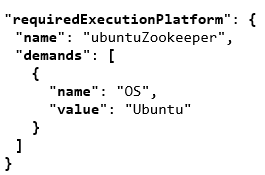
\includegraphics{./Figures/Zookeeper}
	\begin{lstlisting}[caption={Specification of the required platform for Zookeeper component},label={lst:2}]    
	\end{lstlisting}
\end{center}

\noindent It implies that the zookeeper will be executed on a VM running Ubuntu as the operating system and thus that the VM should be provisioned first.

\noindent 

\noindent If we would like to run the zookeeper on Amazon, we would only have to change the provider name of the zookeeper VM. In case of changing from one zookeeper node to a zookeeper cluster, we could use the scale out facilities offered by the DSL. This is similar to management operations that could be created from the imperative script mentioned previously, but in declarative approaches reusability of components is a given feature.

\noindent 

\noindent So, reusability of the application component types and implicit deployment logic (deployment engine deploys the application according to its internal execution rules) are the main advantages of the declarative approaches. Nevertheless, hidden deployment logic also imposes some limitations for the developers, for example, what if the application administrator wanted to change the order of execution for some tasks? This would not be possible due to the deployment engine policies. This pin points the main limitation of declarative approaches: the~lack of flexibility. 

%----------------------------------------------------------------------------------------

\subsection{Discussion}
\label{sec:Discussion}

\noindent As we see from our scenario, imperative approaches are less reusable and involve hard and time-consuming tasks of writing deployment plans \cite{Breitenbuecher2014}, while declarative approaches are less flexible. Another aspect of the deployment phase is the process visibility: in imperative approaches you know exactly how the provisioning and deployment tasks will be performed because you specify the deployment plan yourself, while in declarative the process is hidden from you and in practice you have to imagine it when you design your application topology because components' operations, constraints, capabilities actually represent concrete steps during the provisioning and deployment; also it may be not clear how data is shared between components. 

\noindent 

\noindent One more important aspect that we briefly mentioned before is the dynamic reconfiguration of applications. No matter which deployment automation approach or even combination of them is chosen by the application developers, applications evolve over time and have to be redeployed, often many times. This process should be automated enabling the dynamic reconfiguration of the system, and therefore offering support for what is called ``continuous deployment'': ``Continuous deployment is the practice of continuously deploying good software builds automatically to some environment, but not necessarily to actual users'' \cite{fitzgerald2014continuous}. ~For imperative approaches, this can be achieved by writing additional provisioning and deployment plans and executing them to change the existing application. A drawback of such methodology is that your initial application topology or deployment plan will not be synchronized with changes from additional plans, so if you decided to migrate your application, you would have to replay all plans again in the proper order to reach the same state of the application which means redeployment of the whole application. In declarative approaches, in order to minimize the impact on the running system and thus maximize the application availability, continuous deployment could be achieved by calculating the difference between the previous application topology model and the new one, and then by adapting the running application according to calculated differences as proposed in \cite{FerrySongRCS14}. However, this assumes that the running system is stable. If some virtual machine stopped for any reason, adopting these changes to the previous model would result in the wrong configuration. A simpler scenario would be just to redeploy the whole application, but it is not efficient. A solution to this is to implement the models@run-time architectural pattern. Models@run-time provides an abstract representation of the running application. A change in the running application is immediately propagated to the model of the current system and the same is true for the opposite, any changes to the model are enacted on the running application \cite{FerrySongRCS14}. By using this pattern, application developers can have a consistent view of the system at any time and seamlessly evolve it in the future. To the best of our knowledge, this pattern has been used only in a declarative approach in the context of cloud computing.

\noindent 

\noindent Following the discussion, our proposal for the application provisioning and deployment consists in combining the declarative and imperative approaches: the deployment engine generates the provisioning and deployment plan from the defined application topology model and then the user can analyze it and then has ability to change it before the actual enactment of the plan. Moreover, in case of continuous deployment the same process takes place. For instance, the user changes the topology of an application, an adaptation plan is generated and the user can tune it before the plan will be executed (Figure \ref{fig:solution}). 

\noindent

\begin{figure}[htbp]
	\centering
		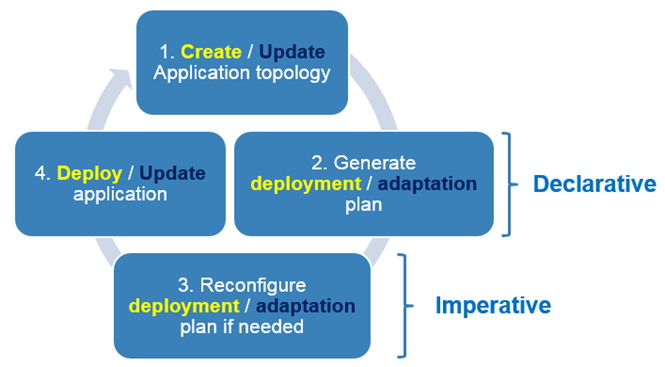
\includegraphics[width=34em]{./Figures/Desired}
		\rule{38em}{0.5pt}
	\caption[Desired Solution]{Desired Solution}
	\label{fig:solution}
\end{figure}

\noindent

\noindent Because imperative approaches often use general workflow languages for the specification of the deployment plan, it would be nice if our plan were expressed using some domain-specific language for modeling workflows.

\noindent In such scenario we preserve reusability of declarative approaches and add flexibility of imperative ones, we have the visibility of the process execution without writing the process ourselves, and we can properly evolve our application and be ready for migration without the issue of replaying a set of workflows or synchronization of our initial application topology with its current state. In addition, this approach results in the reduced time-to-market and development efforts.

%----------------------------------------------------------------------------------------

\section{Research Problem}

\noindent In this work we focus on two challenges: (i) combination of the declarative and imperative approaches to the application provisioning and deployment, and (ii) continuous deployment of cloud applications. Based on this, the research problem may be formulated as follows: 

\begin{center}
"How can we enable both, flexibility and fine-grained control, in the deployment and provisioning of multi-cloud applications, and allow efficient run-time management of such applications?"
\end{center}

\section{Research Questions} 

\noindent The problem addressed by this thesis rises the following questions:

\begin{enumerate}
\item  How imperative and declarative approaches can be combined? Does a combined approach furnish a more efficient and flexible solution?

\item  How to create a DSL for the specification of deployment plans that can be used in combination with declarative deployment topology models, and programmatically by a third party?

\item  How such DSL could be used to support efficient continuous deployment of multi-cloud applications?

\end{enumerate}

%----------------------------------------------------------------------------------------

\section{Research Methodology}
In this section we explain our research methodology and develop a research work plan.

%----------------------------------------------------------------------------------------
\subsection{Methodology}

\noindent The adopted methodology of this thesis relies on a literature survey and design science \cite{von2004design}. Literature survey covers not only publications in scientific journals but also analysis of widely used tools because provisioning and deployment processes relate more to the practical side of computer science than its theoretical underpinnings. Design science guidelines help us in the development of our solution and ensuring that our results are relevant, verifiable and appropriately evaluated.

%----------------------------------------------------------------------------------------
\subsection{Work Plan}
Following the discussion from the Section \ref{sec:Discussion} and, according to the research problem, we can define the initial set up for the research: the approach that we will work on must be declarative, open source and provide support for the continuous deployment. Then, the work plan to answer research questions includes the following steps:

\begin{enumerate}
\item  Analyze state of the art tools and approaches for provisioning and deployment of cloud applications. If the approach is imperative -- which workflow definition language it uses for the specification of the deployment plan?

\item  Choose a declarative approach for the improvement.

\item  Analyze how deployments plans are defined in imperative approaches. Extract common characteristics and limitations of languages used to define deployment plans, and create a domain-specific workflow definition language to specify such plans.

\item  Integrate a chosen approach, including the continuous deployment functionality, with created DSL.

\end{enumerate}

\noindent The rest of the thesis is organized as follows. In Chapter \ref{Chapter2} we analyze current developments in the area of cloud applications provisioning, deployment and runtime management, identify what can be improved and set goals to design our solution. Chapter \ref{Chapter3} describes the design and implementation phases, and in Chapter \ref{Chapter4} we evaluate our solution by performing several deployment experiments. Finally, in Chapter \ref{Chapter5} we conclude our findings and define a road map for further research.

%----------------------------------------------------------------------------------------
% Chapter 1

\chapter{Analysis of the State of the Art} % Main chapter title

\label{Chapter2} % For referencing the chapter elsewhere, use \ref{Chapter1} 

\lhead{Chapter 2. \emph{Analysis of the state of the art}} % This is for the header on each page - perhaps a shortened title

%----------------------------------------------------------------------------------------

\noindent In this section we discuss current research and solutions in the area of cloud applications' provisioning, deployment and management. Plenty of tools and approaches have been developed to address specific challenges in the management of the life-cycle of cloud applications, so the following analysis includes overview of the tools widely used by the industry players for the applications' provisioning and deployment, as well as findings from the latest research in this area. The analysis will lead us to the selection of the tool or approach on which we will focus our research efforts. To make a final selection, first we define a set of requirements which a given approach shall fulfill to be considered as a candidate for improvement. Then, we compare each discussed approach against our set of requirements and identify the final candidate. 

%----------------------------------------------------------------------------------------

\section{Requirements}

\noindent We analyze three areas of applications' provisioning, deployment and management to define our requirements, namely: provisioning and deployment process execution, workflow definition and topology description languages, and runtime application management. Essential requirements were defined in the research questions: the approach must be declarative (R1), open-source (R2) and provide support for continuous deployment (R3).

\noindent 

\noindent \textbf{Provisioning and deployment process execution.}

\noindent We have already discussed declarative and imperative approaches separately and their pros and cons in Section 1. Some tools can offer a mixture of these approaches: deployment workflow is derived from the application topology but the default order of operations and data exchange may be altered with the help of additional custom-written workflows, tasks or by setting of some specific properties in your application topology model \cite{juve2011automating, Breitenbuecher2014}. Tuning the order of operations and data exchange is definitely a useful feature (R4) and ideally it shall be possible to do this via some graphical tool, without writing any additional workflows, or at least with some high-level API. One more aspect here - some approaches install additional software on virtual machines during the deployment phase that may be used for monitoring or software installation. From the user perspective, it is better to avoid any additional software on every virtual machine because the application owner has to pay for the storage, CPU and RAM resources and it may affect the performance of the application. So, another requirement is that approach must be non-invasive: no additional software that is not directly related to the application on virtual machines (R5). Declarative approach requirement (R1) also falls into this category.

\noindent 

\noindent \textbf{Workflow definition and topology description languages.}

\noindent Topology description languages are mostly used in declarative approaches to describe the structure and final state of the cloud application, while workflow definition languages are used in imperative approaches for specifying each step of the deployment plan and their ordering. When we describe the topology of the application we usually think about virtual machines, databases, web servers and other application components. Nevertheless, some tools allow users to compose only virtual machines in their application topology model \cite{juve2011automating, konstantinou2009architecture}. We believe this is not sufficient because then application developers can enforce only the order of the virtual machines' provisioning and do not have any control over the ordering of the software installation and configuration. Such limitation reduces the flexibility of the given approach, so the ability to model full deployment stack (infrastructure, platform and services) by means of the topology description language is important too (R6). In Section 1 we mentioned that imperative approaches often rely on generic workflow definition languages, while offering a language specific to the domain of cloud deployment and provisioning would be more appropriate (R7) as we deal with concrete phases of the cloud applications' life-cycle. 

\noindent 

\noindent \textbf{Run-time application management.}

\noindent Challenges of the run-time applications management such as software updates, scaling, dynamic reconfiguration were discussed in Section 1. From that discussion we came up with requirement about continuous deployment that is related to dynamic reconfiguration of applications. Dynamic reconfiguration includes activities such as scaling and software updates, but in order to better distinguish one approach from another we put an ability to scale applications components as a separate requirement (R8). Last but not least, as we discussed earlier, dynamic reconfiguration may be achieved in several ways and one efficient way to implement it, is by calculating the difference between the running system and a new version of it and then applying only commands related to this difference (R9).

\noindent 

\noindent \textbf{Cross-cutting requirements.}

\noindent Again, following the arguments from the Section 1, all previously mentioned challenges become more complex when application owners want to use multiple cloud providers at the same time for different parts of their application. Such scenario affects all deployment phases and as an example, we may consider application scaling: on a single cloud it means increasing capacity of the server or adding more servers to the same cloud, while in multi-cloud environments we would refer to what is called cloud bursting \cite{amedro2010efficient} -- a situation when there is sudden increase in computation requirements and some resources from the user's local environment or private cloud are offloaded to another cloud provider. This may happen because application providers do not have enough capacity on their private cloud or because increase in computations affects performance of business critical modules of the application, so non-business critical components will be moved to another cloud. Nevertheless, nowadays multi-cloud deployments are essential to avoid vendor lock-in (R10). Another listed challenge was provisioning of resources on IaaS and PaaS levels simultaneously (R11). Open-source requirement (R2) also belongs to the additional requirements category as it does not affect the deployment process anyhow.

\noindent 

\noindent Based on these areas of interest, here is our grouped list of requirements:

\noindent 

\begin{enumerate}
\item  Provisioning and deployment process execution:
\begin{enumerate}
\item  R1 - ``Declarative approach'': provisioning and deployment workflow (plan) must be derived from the application topology model.

\item  R4 - ``Workflow refinement'': it must be possible to change derived workflow at least in terms of the order of operations and data exchange.

\item  R5 - ``Non-invasive'': no additional software (software that you did not define as part of your application) shall be installed on virtual machines to facilitate the application deployment.
\end{enumerate}

\item  Workflow definition and topology description languages:

\begin{enumerate}
\item  R6 - ``Full deployment stack modelling'': it must be possible in the application topology model to describe any types of application components like virtual machines, servers, relationships to allow specification of dependencies on different levels, not only between virtual machines. 

\item  R7 - ``Domain-specific workflow definition language'': the workflow definition language must reflect tasks and behaviors relevant to the area of provisioning and deployment of cloud applications.
\end{enumerate}

\item  Run-time application management:

\begin{enumerate}
\item  R8 - ``Scalability'': it must be possible to scale application components in and out either via API/CLI calls, or topology description updates, or policies.

\item  R3 - ``Dynamic reconfiguration'': it must be possible to reconfigure application during the run-time and update the application topology model or deployment plan according to the new application state.

\item  R9 -- ``Efficient reconfiguration'': dynamic reconfiguration of the application must be performed by applying the necessary modifications to the running system instead of redeploying the whole application. In addition, it is important that the application owner has an overview of the running system, so he can be sure which changes to make. This is essential because components may fail and the system may not be identical to the one that was defined during the design-time, so applying changes to such system will result in the wrong state of the application.
\end{enumerate}

\item  Cross-cutting requirements:

\begin{enumerate}
\item  R10 - ``Multi-cloud'': ``Multiple Cloud delivery model assuming no prior agreement between the Cloud providers and a third party responsible for provider contracting, consumption negotiation, SLA monitoring, inter-provider networking, code and data migration'' \cite{petcu2014consuming}. Although, in our case we do not consider data migration and synchronization.

\item  R11 - ``IaaS and PaaS resources provisioning'': it must be possible to provision resources on different levels of the cloud computing stack.

\item  R2 - ``Open-source''\footnote{ The Open Source Initiative, $  $http://opensource.org/osd}: the code of the project must be freely accessible for use and modification.
\end{enumerate}
\end{enumerate}

%----------------------------------------------------------------------------------------

\section{Tools and Approaches}

\noindent The above set of requirements allows us to start the analysis of different tools and approaches for the provisioning and deployment of cloud applications.

\noindent Some approaches operate only on one level of the cloud stack, for example, they manage dependencies only between virtual machines or between middleware components. Example of such approaches are presented in \cite{juniormodel, konstantinou2009architecture} and \cite{juve2011automating}. 

\noindent In \cite{juniormodel} an automatic model-based approach to software deployment is proposed. It is a declarative approach. The deployment process is derived from UML models based on dependencies between so-called services (components), not virtual machines. One UML model is general and includes application topology view, and another one is provider-specific - includes the name of the provider and credentials. Deployment is performed with a help of 14BIS (a platform to deploy third party software) as a software repository and Chef\footnote{ Chef automation tool, https://www.chef.io/}. During the deployment, a list of recipes (installation scripts) is uploaded to each virtual machine and executed there. This approach is provider independent in terms of infrastructure providers, but it is tied to the deployment service provider - 14BIS platform. Developers can define application topology~and it will be properly deployed, but they can not tune the order of the deployment - a major limitation of declarative approaches. In addition, this approach has no functionality for the run-time phase and no code available for testing purposes, and it is invasive because of usage of Chef.

\noindent 

\noindent The approach presented in\cite{ konstantinou2009architecture} consists of three models: (i) virtual solution model (VSM), which is a set of composable virtual appliance models (virtual images with pre-built configuration points); (ii) VSM is transformed into the virtual solution deployment model (VSDM) that can have some additional cloud-specific properties; (iii) a VSDM is then transformed into virtual solution deployment plan (VSDP) which is responsible for the cloud application provisioning and deployment (Figure \ref{fig:virtual}). 

\begin{figure}[htbp]
	\centering
		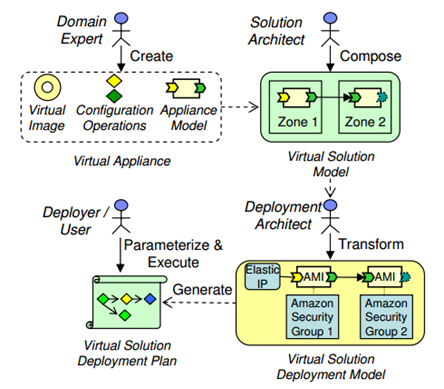
\includegraphics{./Figures/Konstantin}
		\rule{38em}{0.5pt}
	\caption[Virtual Solution Approach]{Virtual Solution Design and Deployment}
	\label{fig:virtual}
\end{figure}

\noindent A few limitations of this approach are: every model must be configured manually by expert users, the only available implementation is proprietary and application topology model (VSM) is based on the composition of pre-built virtual machines, not on the independent software components. Regarding the deployment - details are not covered in the paper but it is based on the research of the deployment patterns and constraints on virtual machine' ports: linkage of ports implies a deploy order dependency. The actual deployment plan is performed by platform-specific workflows (for instance, IBM Solution Assembly Toolkit workflow or Eclipse job manager). So, this is a declarative approach to some extent (Virtual Appliance and Virtual Solution Model), but it requires a lot of human involvement to prepare VMs and all models, and it has the same problem as the previous approach - deployment order can not be changed after VSM is ready. 

\noindent 

\noindent In \cite{juve2011automating} a multi-cloud solution called Wrangler is described. Application topology is described there using specific XML dialect. A topology description is sent to the WRANGLER web-service (multiple interfaces are available: XML-RPC, Python API, command line) which orchestrates provisioning and deployment of the application. Each component may have a bunch of plugins (scripts) which are used for its configuration. The deployment order is decided from DAG-based\footnote{ Directed Acyclic Graph, http://en.wikipedia.org/wiki/Directed\_acyclic\_graph} dependencies in XML document and component groups. Dependencies define the order of VM's provisioning and configuration, and groups are used for systems that require nodes to know about each other. First, all VMs of a group are provisioned (so their IP is known and may be shared with other nodes) and only after that configured. This approach may be attractive because deployment to multiple clouds at the same time is possible, and some run-time commands are available like adding or deleting nodes (no dynamic reconfiguration is possible), and also monitoring of VMs can be done. Nevertheless, it supports only IaaS-level dependencies between components, no code or implementation is available, plugins must conform to a standard set of operations (start, stop, status), serial provisioning of VMs, and this approach is invasive - you have to prepare VMs by installing some additional software before you can use them as part of the topology.

\noindent 

\noindent More advanced approaches allow application developers to define application components and their relationships on all three cloud stack levels (IaaS, PaaS and SaaS) and in addition, they usually allow deployments to multiple clouds simultaneously (although WRANGLER, which was mentioned before, also has such capability) and have more advanced operations for the run-time management (for example, policy-based application management). Two of such approaches are TOSCA and Apache Brooklyn.  

\noindent 

\noindent TOSCA \cite{INPROC-2013-45} application topologies can be processed in an imperative or declarative way. Imperative processing relies on management/build plans (workflows) which are typically implemented by the application developer. Plans define required services in an abstract way, concrete endpoints are bound from implementation artifacts (e.g., SOAP Web services, REST, scripts) of application components (nodes). Plan Portability API allows access to topology and instance information, for instance, property values of nodes and relationships (runtime info: ports, IP of VMs). Credentials and configurations (for instance, machine size) are passed to the Build Plan as inputs. During the run-time, the workflow engine enacts operations of the build plan and in that way the application is provisioned and deployed. Dynamic reconfiguration may be theoretically achieved by writing new plans and running them on top of the existing application, but if many such plans will be written, eventually it will be not possible to maintain such application. Declarative processing of applications in TOSCA is possible with Plan Generator \cite{Breitenbuecher2014} which takes a topology with all artifacts (deployment and implementation) as input and produces fully executable workflow that can be adapted afterwards. Plan Generator was a separate tool at the time the paper was published and we were unable to find any more recent information about it. The order of the provisioning is based on the types of Relationship Templates: if node A is ``hostedOn'', ``dependsOn'', ``runsOn'' node B, then node B must be provisioned first. Relations of types ``calls'', ``invokes'', ``connectsTo'' require both nodes to be instantiated before the relation can be instantiated. In addition, TOSCA simple profile in YAML \cite{TOSCA-Simple-Profile-YAML-v1.0}is under development that will allow declarative provisioning and deployment, probably based on the repository of the node and relationship types. The main limitation of TOSCA is that it is not possible to dynamically reconfigure the application.

\noindent 

\noindent Another available system is Brooklyn\footnote{ Apache Brooklyn, $  $https://brooklyn.incubator.apache.org/} which is used for deploying and managing distributed applications. It is an open-source system, it supports multi-cloud deployments and also the definition of PaaS-level components in the application topology model. Application topology is described in YAML or JAVA blueprints via entities (pieces of code) which can have operations, attributes, policies and sensors (for monitoring). Run-time operations such as scaling are available, including monitoring and policy-based management of the application. The deployment order is based on the hierarchical tree of entities (each entity has a parent and may have children, except application entity that is a top-level entity) and is done in parallel. Default provisioning order may be customized with the help of tasks if the user needs to defer the start of one entity before another one reaches some state and can share its values for instance. The deployment execution status is visible to operators. A repository of entities is available which makes it easier to construct applications. Limitations of the approach include: (i) it is not possible to change topology (and thus deployment order) with regard to the underlying schema (parent-child relationships) and (ii) it is not possible to dynamically reconfigure the application.

\noindent 

\noindent Next stage of the improvement to deployment processes brings the capability to update applications dynamically during their run-time. A few systems that have such feature are CloudMF, Cloudify and SmartFrog.

\noindent 

\noindent 

\noindent CloudMF consists of a cloud modelling DSL called CloudML which allows abstract description of the desired application topology along with the specification of its provisioning and deployment, and a models@run-time environment for the enactment of the provisioning, deployment and adaptation of the application. Models@run-time is a unique feature of CloudMF as authors state in their paper \cite{FerrySongRCS14}: ``.. the work of Shao \cite{ShaoWeiWM10} was a first attempt to build a models@run-time platform for the cloud, but remains restricted to monitoring, without providing support for configuration enactment. To the best of our knowledge, CloudMF is thus the first attempt to reconcile cloud management solutions with modeling practices through the use of models@run-time.'' Models@run-time environment provides the causal connection between the running system and application topology model. So, after the initial application was deployed, application owners can change the application topology model and issue a deploy command. After that the deployment engine will compute required changes and update the running application. Update in this case means only performing the necessary modifications such as the  deployment of new components thus, there is no need to redeploy the whole application. From the other side, if some VM crashes, this information will be automatically populated in the in-memory application topology model. The deployment order in the CloudMF is based on the engine policies and components' requirements and capabilities. For instance, a web server requires a database to operate properly, this means that the database will be installed and started before the web server. CloudMF is also a declarative approach, so it is not possible to tune the deployment order to the user's specific needs. In addition, scalability functionality is not yet implemented properly: if it is required to create one hundred VMs of the same type, the developer will need to describe each of them. In addition, deployment tasks are executed sequentially, which is not suitable for large-scale applications deployment. The project is open-source and the code is available on Github\footnote{ CloudML, https://github.com/SINTEF-9012/cloudml}.

\noindent 

\noindent Another similar tool called Cloudify\footnote{ Cloudify, $  $http://getcloudify.org/} focuses on cloud orchestration and automation. A topology is described in a blueprint that is inspired by the TOSCA YAML profile and includes application nodes, workflows and relationships. From blueprints, developers can create deployments (i.e., blueprints enriched with input data), and then run built-in or custom workflows to deploy or undeploy the application. Provisioning and deployment are done with the help of a stateful orchestrator called Manager that runs automation processes described in workflows. Each task of the workflow is delegated to Agents: manager side agents are responsible for the provisioning, and application side agents - for the deployment of different components. Finally, the actual execution of each task is performed with the help of Plugins: scripts, Chef, Puppet or Docker tools. Regarding the order of execution, default order is based on relationships of nodes (all nodes may be started in parallel) and built-in lifecycle of a node: create node, preconfigure relationship, configure node, post-configure relationship, start node, install agent workers and required plugins, establish relationship, start monitoring. Any node may have custom workflows that will change the default execution order. Multi-cloud support, a repository of blueprints and some plugins are available only in premium version what makes this approach less attractive for the users. Regarding the dynamic reconfiguration capabilities of the Cloudify -- in some places in the documentation and a few use cases that highlight the benefits of Cloudify, it can be found that such feature is available. At the same time, it is not clear what they mean by the dynamic reconfiguration (seems to focus mainly on the scaling of the application) and no details are provided about how exactly this can be done.

\noindent 

\noindent In\cite{Frog}, an extension to SmartFrog framework \cite{goldsack2009smartfrog} is presented which allows multi-cloud deployments and application adaptations during the run-time phase. Each application component is modeled as an object whose lifecycle events correspond to specific actions like Deploy, Start, and Terminate. The deployment manager can link the lifecycle of different components by such constructs as compound (start and terminate components together), parallel (start components concurrently and let them evolve independently) and sequence (a component start only after previous component terminated) and this linking will determine deployment plan. Later on, when some component has to be moved to another cloud for instance, deployment manager can query Metadata database to determine dependencies of this components, and based on the query result, adaptation is executed. Details are not clearly explained: in \cite{goldsack2009smartfrog} researchers simply mentioned that some programs must interact with SmartFrog framework to handle application adaptation scenarios. In addition, in \cite{Frog} two evaluation scenarios that were presented focused on migration of services from one cloud to another, so it seems like the dynamic reconfiguration is possible but only in terms of the changes to the location of services, not to the underlying services architecture. Other drawbacks of this approach are: each VM runs SmartFrog daemon, so the approach is invasive, and it is not possible to refine the workflow - deployment plan will be based on the chosen deployment construct (compound, parallel, sequence). 

%----------------------------------------------------------------------------------------

\section{Summary}

\noindent After analyzing each approach we summarize our findings in Table \ref{tab:1}. Requirements analysis was simplified to save some space in the descriptions of each approach, while Table \ref{tab:1} shows exactly how all approaches satisfy our list of requirements. Such requirements as ``Declarative approach'', ``Dynamic reconfiguration'' and ``Open-source'' were defined as essential requirements, so they are highlighted. ``N/A'' mark means that this requirement is not applicable to the given approach or there is no definite answer, for instance when some approach was not positioned as proprietary solution but at the same time we could not find a source code for it. ``yes*'' mark means that requirement is satisfied but under certain conditions. Finally, ``?'' mark refers to the situation when the approach claims to satisfy the requirement, but we could not find the information about how a given feature is implemented.

\noindent

\noindent Starting from the ``Declarative approach'' requirement we can see that all approaches satisfy this requirement, except TOSCA, which can offer declarative deployments with help of the Plan Generator as discussed before, but we were unable to get the code of the Plan Generator or to find its implementation. Next essential requirement is ``Dynamic reconfiguration'': only CloudMF, Cloudify and extended SmartFrog framework can provide such feature, so at this point five out of eight approaches can be eliminated. It is not clear what is meant by the dynamic reconfiguration in Cloudify and SmartFrog approaches: scaling of the application, relocation of virtual machines from one cloud provider to another, changing the parameters of some application components or changes to the application architecture, so they receive lower ranking than CloudMF with regard to the ``Dynamic Reconfiguration'' requirement. As for the ``Open-source'' requirement, all three approaches are open-source projects, but Cloudify offers such feature as multi-cloud deployments only under subscription, so we can eliminate it too. Between CloudMF and SmartFrog approaches we choose CloudMF because it is non-invasive and clearly satisfies such requirements as dynamic and efficient reconfigurations.

\begin{center}
	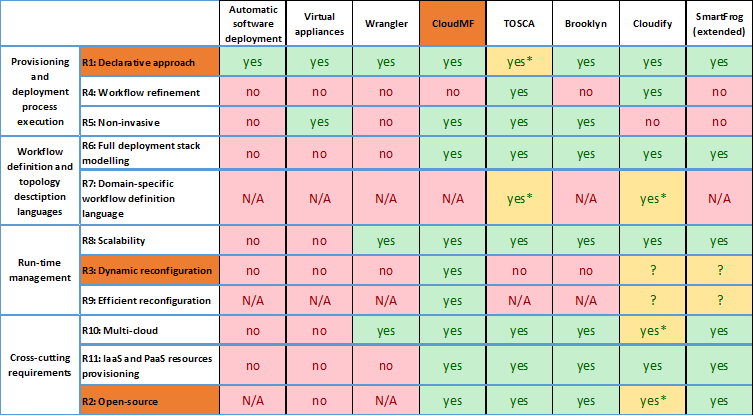
\includegraphics[width=38em]{./Figures/Comparison}
	\begin{table}[htbp]
    \caption{Comparison of Provisioning and Deployment Approaches}
    \label{tab:1}
	\end{table}
\end{center}


\noindent One more observation from the comparison is that there is no domain-specific language for provisioning and deployment of cloud applications. Cloudify relies on a so-called graph framework to specify custom workflows, but there is no details about it in the documentation right now, and looks like they went for such solution not because of some domain-specific semantics of the framework, but rather because it allows to parallelize tasks in an easy way through concrete API. As for TOSCA which currently uses BPEL for the definition of deployment plans, BPEL can be considered as domain-specific language for business process modelling, but not specific for the deployment domain. While it could be used in the deployment domain, if deployment actions were expressed as services, it seems too powerful and complex. 
% Chapter 1

\chapter{Implementation} % Main chapter title

\label{Chapter3} % For referencing the chapter elsewhere, use \ref{Chapter1} 

\lhead{Chapter 3. \emph{Implementation}} % This is for the header on each page - perhaps a shortened title

%----------------------------------------------------------------------------------------
\noindent In this chapter we highlight our design choices and implementation details of the proposed solution.

\section{Domain-specific Language}


%----------------------------------------------------------------------------------------

\noindent After the selection of the suitable declarative approach for building our prototype we can start with the creation of the domain-specific language that shall allow the specification of the provisioning and deployment plans. The motivation here is that there are languages available that allow the specification of workflows (plans), but they are too generic. We want our language to be specific to the deployment and provisioning domain. Thus, it is important to identify language constructs that are relevant to this domain and also to the specification of the deployment plan execution logic. From the other side, to release engineers from learning new notations, our DSL shall be compliant to the main workflow definition languages, such as PetriNets\footnote{ Petri Nets World, $  $http://www.informatik.uni-hamburg.de/TGI/PetriNets/}, BPMN\footnote{ BPMN 2.0 standard, $  $http://www.omg.org/spec/BPMN/2.0/} or WS-BPEL\footnote{ WS-BPEL 2.0 standard, $  $http://docs.oasis-open.org/wsbpel/2.0/OS/wsbpel-v2.0-OS.html}, or UML Activity Diagrams\footnote{ UML 2.0 standard, $  $http://www.uml.org/\#UML2.0}. For the sake of clarity we shall state that BPMN and UML are more related to the workflows design phase, while WS-BPEL - to the workflows implementation phase, and PetriNets may be used for both. We are interested in the design and implementation phases, so we analyze them together.

\noindent 

\noindent A short overview of these languages:

\begin{enumerate}
\item  PetriNets is a graphical and mathematical modeling tool that can be used in many different systems \cite{murata1989petri}: concurrent, asynchronous, nondeterministic and distributed. PetriNets may be used by theoreticians to model systems and analyze them as well as by practitioners in real-world scenarios to execute some processes. PetriNet itself is a directed graph with two kinds of nodes -- places (circles) and transitions (rectangles), and arcs that may lead either from place to transition or from the transition to a place. Places are holders of tokens and transitions are consumers and producers of tokens. Tokens are used to enable the execution of events (transitions). By simulating a movement of tokens from one place to another, the execution of a process/workflow may be analyzed.

\item  BPMN stands for Business Process Model and Notation and is a standard to represent processes in virtually any kind of organization \cite{chinosi2012bpmn}. Its primary goal is to provide a notation for the business processes that can be clearly understood by the business and technical users at the same time. A business process is represented in a Business Process Diagram which consists of Flow Objects (Events, Activities, Gateways) which determine behavior of the business process; Connecting Objects (Sequence Flow, Message Flow, Associations) to connect objects to each other; Swimlanes (Pools and Lanes) for grouping a set of elements; Artifacts (Data Object, Group, Annotation) for providing additional information. BPMN 2.0 provides the ability to model new sets of processes such as Orchestrations, Choreographies and Collaborations and puts more emphasis on the importance of Data.

\item  WS-BPEL is a language for the specification of the executable and abstract business processes, based exclusively on Web Services. It defines the model and grammar to describe the behavior of a business processes. Executable business processes model actual behavior of a given participant of the process, while Abstract business processes serve a descriptive role and may be used in more than one use case. The specification consists of partnerLinks -- to defined different parties involved in the business process, variables -- to represent data, faultHandlers -- activities that must be performed in case of errors in the process and the process itself. The process in turn consists of different activities: some of them are directly linked to web services like receive, reply, invoke; others define the structure and ordering of the other activities in the process - like sequence, flow, scope, wait, forEach, while and more.

\item  UML Activity Diagram is part of the UML (a graphical notation for modeling object-oriented systems) and shows activities and actions to describe workflows   \cite{JOT:issue_2003_07/column3}. The diagram itself consists of nodes (action, structured, control and object nodes) and edges (control and object flow edges). In addition to that, different kinds of events may be added. 
\end{enumerate}

\noindent 

\noindent It is important to mention here that pure PetriNets cannot be compared with BPMN or UML Activity Diagrams as they do not have any way to represent data objects, so when we talk about PetriNets we actually refer to their variant called Colored PetriNets \cite{jensen1991coloured} in which it is possible to represent any kind of data, time constraints and more.

%----------------------------------------------------------------------------------------
\subsection{Selection of the Language Constructs and Language Representation}

\noindent All of these languages have similar expressive power \cite{geambacsu2012bpmn, storrle2004semantics, hinz2005transforming}, so it is possible to describe most workflows in any of them, although the effort to do that will differ from one language to another. By the similar expressive power we mean that they all share (under different names, of course) such constructs as actions, control and data nodes, control and data flows, and different kinds of events. Control nodes and flows are used to determine the ordering of actions (for instance, concurrent execution of tasks, which is essential for the deployment of large-scale cloud applications), data nodes and flows are used to pass objects from one action to another, and actions themselves -- for the actual execution of the workflow. In addition, events may be used to handle errors or interactions with users, or communication between different workflows. 

\noindent 

\noindent In practice, as stated in \cite{zur2008much}, some constructs of these languages may not be needed: ``... the complexity of BPMN in practice differs considerably from its theoretical complexity. This, in turn, suggests that future research should take this distinction into account when considering BPMN's expressive power, complexity or other features or characteristics''. That is why from the list of constructs that we just discussed, we have to choose which of them are relevant to the deployment activities and are useful to define the proper ordering of tasks in the deployment plan.

\noindent 

\noindent A small set of language constructs could also be justified by the analysis of the deployment approaches that usually have the same set of common tasks such as download, install, configure, start, and stop. The need for events, error handlers, and some types of control nodes is quite questionable in the context of the deployment process:

\noindent 

\begin{enumerate}
\item  as long as the application topology model is ready (declarative approaches) or deployment plan is created (imperative approaches), no interaction with the user is usually expected during the execution of the deployment plan, so receive events are not needed; timer events could be useful but in most cases they may be eliminated by the proper synchronization of different tasks. And even if they are really needed - users of our DSL would be able to represent them as normal tasks (probably with a specific name ``timer'') without the need to add more constructs to the DSL itself.

\item  as for error handling events, we argue that errors during the deployment plan executions happen most often because of improper design of the application topology model, so it is better to fix the model and rerun the deployment, rather then handle errors on the fly. In case error happenned because of another reason (maybe downtime of the cloud provider service), error handling events would still be useless, most probably, because error of one component could lead to the missconfiguration of a bunch of other components. Moreover, even if application operators had an opportunity to handle errors on the fly, the installation of other components that depend on the failed one could time out or make the whole process infinitevily long, if more than one component failed. We believe the deployment process, or at least parts of it, shall have transactional nature -- either succeed or fail. In addition, handling error scenarios is out of scope of this work.  

\item  as for control nodes, tasks such as fork and join are definitely useful for concurrent execution, while it is hard to justify the need for decision and merge nodes because deployment process is a well-planned activity and there shall not be place for any ambiguities.

\item  the need for recurring actions (for and while loops) is also questionable: during the deployment developers may think of recurring actions when it is required to provision a bunch of identical virtual machines, but in that case running such installation in a loop would not make sense because it would be sequential execution and would take a lot of time, so in such case parallel execution is the way to go.

\item  one more observation that was made during the analysis of the deployment tools and approaches - we do not need asynchronous invocation of actions as one task shall not be started before the previous one completes (unless tasks are independent - then we can run them in parallel, but still in a synchronous mode). For instance, installation of the web server can not be started before the virtual machine has been provisioned, so there is no reason to invoke provisioning task asynchronously and continue the deployment process while provisioning task is running.
\end{enumerate}

\noindent 

\noindent Following this discussion, our initial language constructs set may consist of the following elements: 

\begin{enumerate}
\item  control flow to trigger tasks in the deployment plan

\item  data flow to exchange objects between tasks

\item  a task/action node that would represent all kinds of deployment operations

\item  object node to save some variables

\item  start and stop nodes

\item  fork and join nodes to parallelize and synchronize execution of multiple independent tasks

\item  grouping node to execute a set of identical tasks in parallel can be very useful in large-scale applications to keep the deployment plan readable
\end{enumerate}

\noindent Every workflow language mentioned previously contains such set of constructs, so any of them could be used to create our DSL. Nevertheless, these languages were not designed for the same purpose. BPMN is better known in the business world. BPEL, to some extent, is an executable version of the BPMN \cite{ouvans2006bpmn}, so it is mostly known to developers of the business process applications. In addition, BPEL relies exclusively on Web Services as we stated before, while deployment process has little to do with Web Services (except maybe establishing connections to the cloud provider). Finally, PetriNets and UML Activity diagrams are both very well-known modeling tools and are used in many different domains, but we believe that UML Activity Diagrams are easier to read or to learn, and more familiar to developers what is quite important in the context of deployment tools.

\noindent 

\noindent Based on such observations and assumptions we decided that DSL for the deployment and provisioning shall be similar/compliant to UML Activity Diagrams.

%----------------------------------------------------------------------------------------
\subsection{Metamodel of the Provisioning and Deployment DSL}

\noindent To formalize our DSL we refer to the software development paradigm called model-driven engineering (MDE) \cite{kent2002model}. In MDE, models (representations of the system) are central artefacts of a system implementation process. Such models have to be ``written'' in a particular way, dictated by their abstract syntax. This syntax is defined in the metamodel -- ``a model of a model''. Thus, the creation of the deployment DSL shall start from the creation of its metamodel.

\noindent 

\noindent UML Activity Diagrams have more components than the ones we outlined before for our language, so we take a subset of their meta-model for the DSL, which is represented in in the Figure \ref{fig:Metamodel} in the Ecore format\footnote{ Ecore meta-model, $  $http://download.eclipse.org/modeling/emf/emf/javadoc/2.9.0/org/eclipse/emf/ecore/package-summary.html\#details}. The description of each element, along with their graphical notation can be found in Table \ref{tab:2}. ExpansionRegion and ExpansionNode do not have graphical notation in the current version of the DSL because we did not use them in our experiments (the reason is explained later), but in general ExpansionNode is identical to other object nodes and ExpansionRegion has a bit different representation that can be found in the UML specification.

\noindent 

\begin{figure}[htbp]
	\centering
		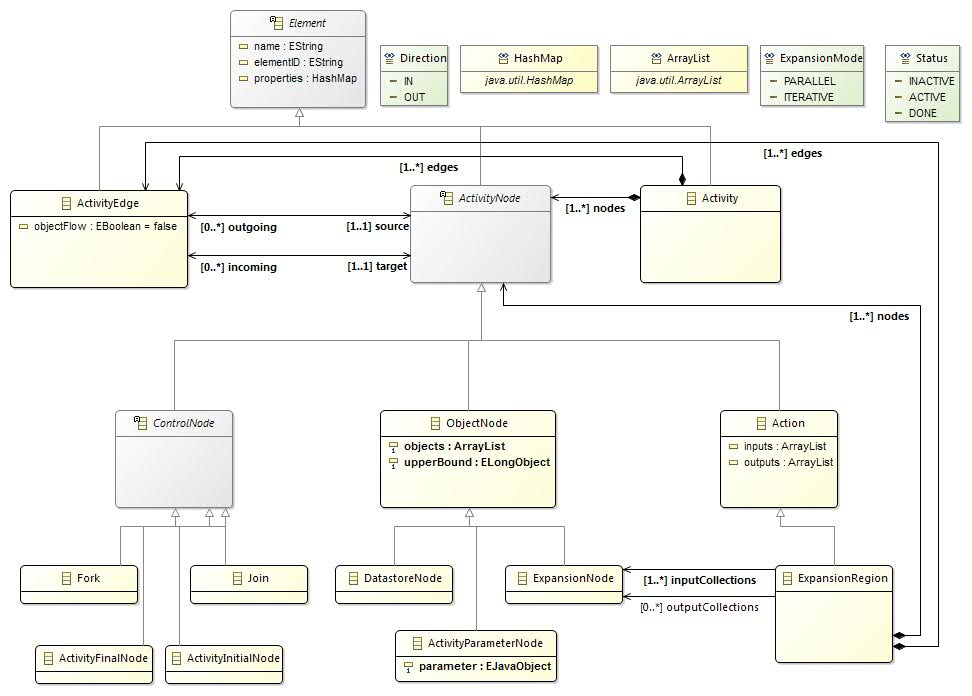
\includegraphics[width=38em]{./Figures/UML_Activity_mine_class_diagram}
		\rule{38em}{0.5pt}
	\caption[DSL Metamodel]{Metamodel of the DSL for provisioning and deployment of multi-cloud applications}
	\label{fig:Metamodel}
\end{figure}

\noindent 

\noindent Moreover, below is the list of the UML Activity Diagram constructs that we skipped with some explanations why we skipped them:

\begin{enumerate}
\item  ActivityGroup: generic construct to group nodes or edges, no need for it except ExpansionRegion which we use. ExpansionRegion is one of the subclasses of ActivityGroup.

\item  Pin: used when object is passed only between two actions, as a combination of data and control flows.

\item  CentralBufferNode: very similar to DatastoreNode, but can not connect directly to actions, acts as a storage place for other object nodes, so it is not needed.

\item  Merge and Decision nodes: see discussion above.

\item  FlowFinalNode: could be useful to stop parallel flows and avoid join nodes in some cases, but currently we consider it to be not very significant and have not. included it in the DSL

\item  ActivityPartition: subclass of ActivityGroup, often corresponds to organizational units in business model, not needed in the deployment plan.

\item  ParameterSet: a complete set of inputs and outputs to activities, may be used in scenarios with multiple activities and we work only with one activity.

\item  InterruptibleActivityRegion: used to handle exception events that we decided not to include.

\item  ExecutableNode: abstract class for nodes that may be executed, used as an attachment point for exception handlers in UML Activity Diagrams, so we do not include it.

\item  StructuredActivityNode: it is another abstraction of ActivityGroup, as we stated before we use only ExpansionRegion to group multiple similar actions and execute them sequentially or in parallel.

\item  SequenceNode: a node that can execute internal actions in sequence, we may use ExpansionRegion in such situations.

\item  LoopNode: we decided to avoid using loops.

\item  ConditionalNode: node that represents exclusive choice that we do not need.

\item  ExceptionHandler: see discussion above.
\end{enumerate}

\noindent To have even better understanding of the DSL, Figure \ref{fig:simplified} depicts simplified deployment plan of the storm cluster with one Supervisor node, using the described graphical notation of the language constructs.

\noindent The metamodel of our language is defined as a set of Java classes\footnote{ DSL for provisioning and deployment of multi-cloud applications, $  $https://github.com/SINTEF-9012/cloudml/tree/Maksym/deployer2/src/main/java/org/cloudml/deployer2/dsl}. In addition to that, we created an internal DSL to abstract low-level operations with language constructs. Internal DSLs (or embedded DSLs) are DSLs represented within the syntax of a general-purpose language - Java in our case \cite{fowler2010domain}. The usage of the internal DSL helps to reduce the number of possible errors during the creation of the deployment plan, and allows manipulations on the deployment plan. In addition, internal DSL could be used by the third party applications to adapt deployment plans. 

\begin{center}
	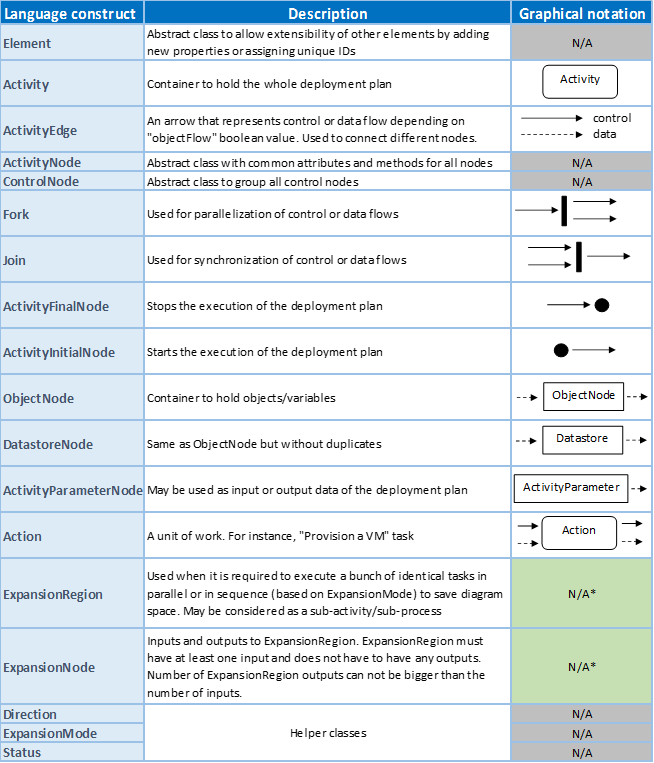
\includegraphics[width=38em]{./Figures/UML_table}
	\begin{table}[htbp]
    \caption{Description of the DSL Metamodel}
    \label{tab:2}
	\end{table}
\end{center} 

\begin{figure}[htbp]
	\centering
		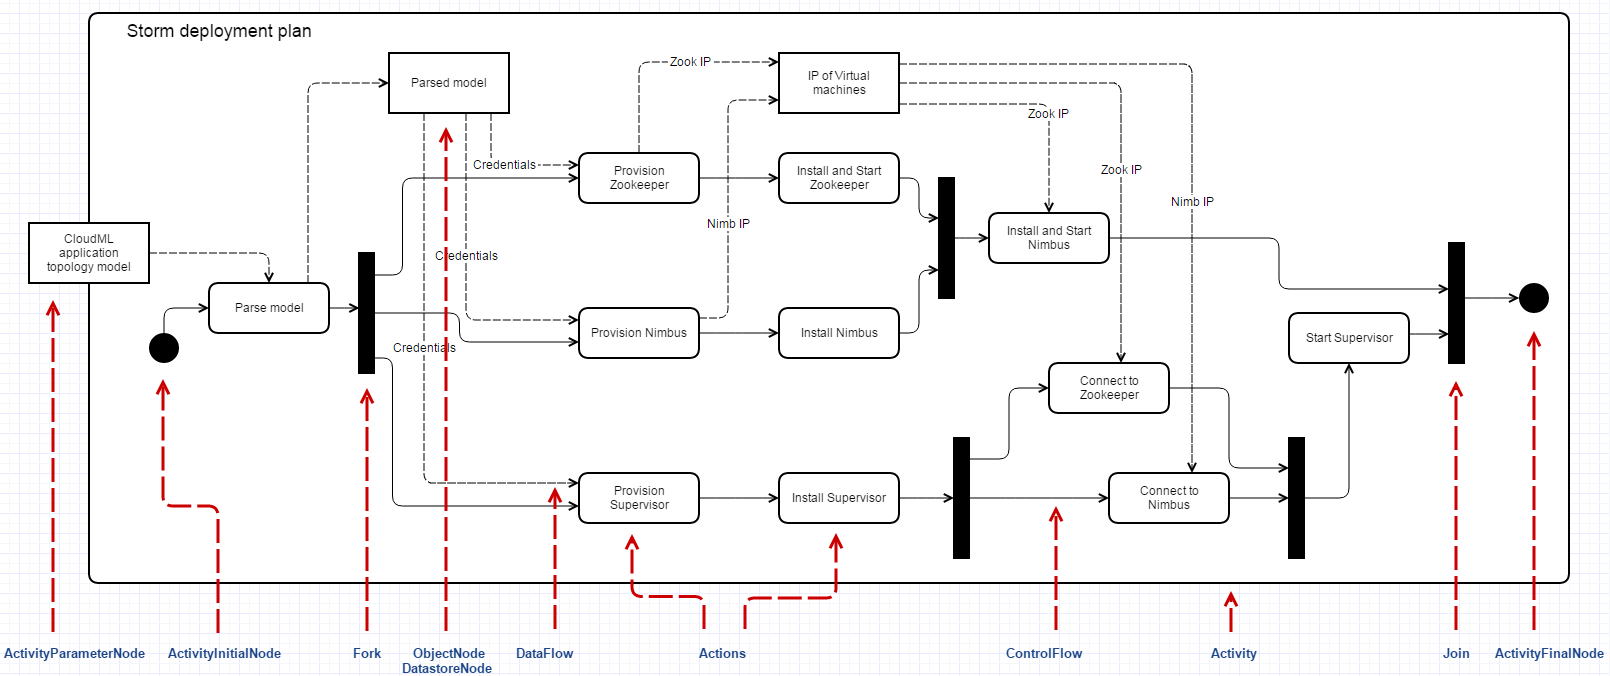
\includegraphics[width=38em]{./Figures/DSL_examplified}
		\rule{38em}{0.5pt}
	\caption[Storm Cluster Simplified Plan]{Simplified deployment plan of a storm cluster}
	\label{fig:simplified}
\end{figure}

%----------------------------------------------------------------------------------------
\subsection{Java Deployment Plan Builder as an Internal DSL}

\noindent To make things clearer, let us consider deployment DSL constructs in the space of our initial example - deployment of the storm cluster. The whole deployment plan for the storm application will be represented as an Activity and can be created with the help of the internal DSL as follows:

\begin{center}
	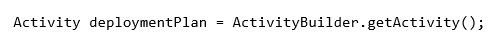
\includegraphics{./Figures/Get}
	\begin{lstlisting}[mathescape,caption={Deployment plan declaration},label={lst:3}]
	\end{lstlisting}
\end{center}

\noindent which will create an empty activity without any nodes or edges, so we can add nodes and edges to it. The deployment plan needs to start its executions at some point, so we start from the creation of the starting point:

\begin{center}
	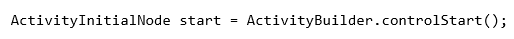
\includegraphics{./Figures/Start}
	\begin{lstlisting}[mathescape,caption={Activity initial node},label={lst:4}]
	\end{lstlisting}
\end{center}

\noindent which creates an initial node with one outgoing edge and adds this node and edge to the ``deploymentPlan'' that we created before. The first thing that has to be done during the deployment is the provisioning of virtual machines. We have three of them, so it is good to run provisioning in parallel, thus we have to create a fork node and three action nodes:

\begin{center}
	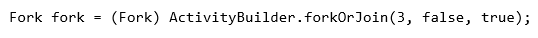
\includegraphics{./Figures/Fork}
	\begin{lstlisting}[mathescape,caption={Fork or Join node},label={lst:5}]
	\end{lstlisting}
\end{center} 

\noindent ``forkOrJoin'' method has three parameters: number of parallel edges, boolean to state if we are dealing with data or control flow, and boolean to decide if we want to create Fork or Join node. Fork node has one incoming and multiple outgoing edges and Join  the opposite: multiple incoming and one outgoing, other than that there is no difference between these two nodes. Both fork and join nodes may be dealing with only data flow or only control flow. The following situations are not allowed by the UML semantics: an incoming edge is a data edge and the outgoing edges are control edges - that is why we need second parameter. Moreover, the first parameter simply tells how many outgoing or incoming, data or control flow edges needs to be created. When fork with all edges is ready, we have to create three provisioning actions and connect them with Fork node, and also connect fork node with start node, because currently it is just a node that belongs to activity and not connected to anything. Actions:

\begin{center}
	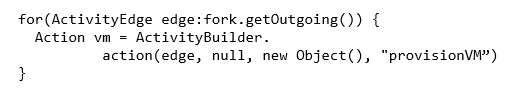
\includegraphics{./Figures/Action}
	\begin{lstlisting}[mathescape,caption={Action node},label={lst:6}]
	\end{lstlisting}
\end{center} 

\noindent ``action'' method has four parameters: incoming control edge, incoming data edge, incoming object and the name of the action. Every action must have an incoming control edge, it may also have incoming data edge (that is why we put null as a second parameter), it also may have input data and definitely some name. Regarding input data, if we think about real deployments every action will have some input: it may be credentials to the cloud provider, credentials to connect to specific VM, name of the command to invoke, shell script or anything else. In the code above, we iterate over outgoing control edges from the fork node and use them as incoming edges to every action, so action are already connected to the fork node. As we mentioned before, we also need to connect fork and start nodes:

\begin{center}
	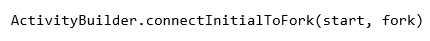
\includegraphics{./Figures/Connect}
	\begin{lstlisting}[mathescape,caption={Connecting two nodes},label={lst:7}]
	\end{lstlisting}
\end{center} 

\noindent This method obviously connects ActivityInitialNode with Fork node, and in addition it performs some more work with the deployment plan. Additional work includes validations that start and fork nodes are connected properly, for instance, if fork node had an incoming edge, then no need to create another edge for a start node. Basically, every method in the ActivityBuilder class that starts with a ``connect'' word performs similar kinds of validations.

\noindent 

\noindent Usually, after provisioning of virtual machines is done, IP addresses of these machines would be needed for further configuration. That is when data flow and object nodes come into play. In the scenario of storm deployment, IP address of Zookeeper VM is needed for configuration of Nimbus and Supervisor components, and IP address of Nimbus VM is needed for the configuration of Supervisor. We can save them all in one place for convenient retrieval. For this we have to create a Join node to synchronize data flows from ``provisionVM'' actions and then Object node to store IP addresses. An assumption here that all provisioning actions are gathered in one list:

\begin{center}
	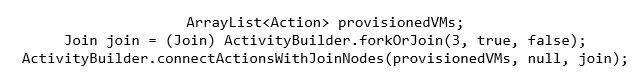
\includegraphics[width=38em]{./Figures/Join}
	\begin{lstlisting}[mathescape,caption={Join node},label={lst:8}]
	\end{lstlisting}
\end{center} 

\noindent Recalling parameters of the ``forkOrJoin'' method, the second parameter means that we are dealing with data flow, and the third - that we want to create a Join node, not Fork node. Then, ``connectActionsWithJoinNodes'' method has three parameters: an array of actions, Join node with control edges and Join node with data edges. In most cases the user would want to connect a set of actions with a Join node of the specific type (with control or data edges), so one parameter would be null, but in case both data and control flow from actions must be synchronized ~- it is possible to do that with this method. A caution for this method: number of actions must not be bigger than the number of incoming edges to Join node, ideally it should be the same. If it will be smaller - you shall remember that there are some edges left in the Join node that do not have any source node and you need to handle them later. What is left after previous calls - to create an Object node and connect it with Join node (Listing \ref{lst:9}). ``objectNode'' is one method to create different kinds of object nodes (Parameter, Datastore, Expansion, Object) with different possible configurations of edges (In, Out, InOut, NoEdges). The first parameter is object node name, second - node type, third - edges configuration.

\begin{center}
	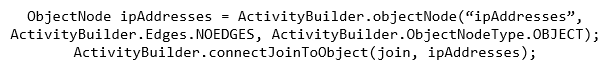
\includegraphics[width=38em]{./Figures/Object}
	\begin{lstlisting}[mathescape,caption={Object node},label={lst:9}]
	\end{lstlisting}
\end{center} 

\noindent Moreover, after creating object node we connect it to the Join node that was created before. One more thing, we did not mention yet how objects are passed between nodes. Currently we are creating a deployment plan, but IP addresses may be saved only after plan execution. So, assuming we have a provisioning action that has one output object with IP address of the provisioned virtual machine, and we have an Object node to store that IP, the process may look like this:

\begin{center}
	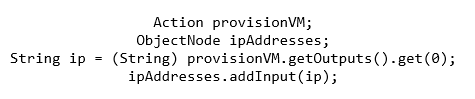
\includegraphics{./Figures/IP}
	\begin{lstlisting}[mathescape,caption={Adding data to the Object node},label={lst:10}]
	\end{lstlisting}
\end{center} 

\noindent So far we have shown how to create different kind of nodes and how to connect them. Concerning the storm example, we created a part of the deployment plan where all virtual machines are provisioned and their IP addresses are saved in one Object node for later retrieval. In a similar fashion we can create nodes and edges for all other installation and configuration commands and finish our deployment plan. Important note regarding ActivityBuilder class - for now it does not have any methods for manipulation on ExpansionRegion. Because we are working with CloudML and it does not have any constructs to group a number of tasks yet, we did not implement ExpansionRegion helper methods in the ActivityBuilder class, but it can be used on its own and added to the deployment plan like this:

\begin{center}
	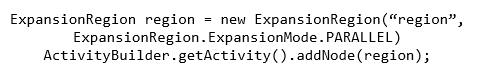
\includegraphics{./Figures/Region}
	\begin{lstlisting}[mathescape,caption={Expansion Region node},label={lst:11}]
	\end{lstlisting}
\end{center} 

\noindent After the generation of the deployment plan, it is important to check if we have not missed anything and everything is properly connected. For that we created a deployment plan validator (ActivityValidator.java class) which checks our model according to the following rules:

\noindent \begin{enumerate}
\item Check if all edges have source and target nodes. Edges can not point to nowhere or come from nowhere.

\item  Check if control edges do not have any kind of ObjectNode as source or target.

\item  Check if all nodes have incoming and outgoing edges to avoid control or data flows that do not lead to the final node. Exceptions here: ActivityFinalNode, ActivityInitialNode and ActivityParameterNode - all of them must have only one edge.

\item  Check if Action nodes have at least one incoming and at least one outgoing control edge because they must be triggered and lead to some other node

\item  Check if source nodes of incoming edges do not match with target nodes of outgoing edges of a given node to avoid cycles. Unfortunately, this rule does not check if there are bigger cycles in the deployment plan, like node number ten points back to node number one.

\item  Check if the activity has initial and final nodes to make sure it can be started and will be terminated eventually.

\item  Check if the activity has only one initial and only one final node to avoid ambiguities or conflicts during the deployment plan execution.
\end{enumerate}

%----------------------------------------------------------------------------------------
\section{Deployment Process} 

%----------------------------------------------------------------------------------------
In this section we explain in details how the deployment process is performed along with the usage of our DSL during the process execution.

\subsection{Introduction} 

\noindent A DSL by itself is useless unless it is used in conjunction with a deployment engine, so the next step is to integrate CloudML with our DSL to enable a transparent deployment process. The integration in this case means the transformation of the CloudML application topology model into the deployment plan - activity diagram with different nodes and edges, and then proper execution of such plan. Following an MDE approach, the transformation is defined at the metamodel level. This means that such an approach is generic and can be used to transform any CloudML model into a deployment plan as long as it conforms to the metamodel. A general idea of the transformation is depicted on Figure \ref{fig:high}.

\noindent 

\begin{figure}[htbp]
	\centering
		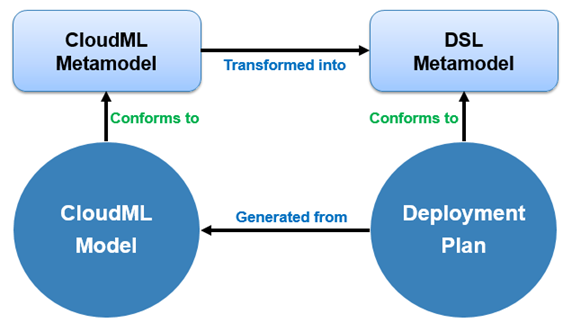
\includegraphics[width=32em]{./Figures/Transformation}
		\rule{38em}{0.5pt}
	\caption[High-level Transformation]{Models transformation (high-level)}
	\label{fig:high}
\end{figure}

\noindent 

\noindent The deployment plan shall represent every command that is executed during the deployment process and all dependencies between those commands to execute them in the proper order. The plan is generated according to the internal rules of the deployment engine (CloudML in our case) but generated sequence of commands might not suit specific needs of the user. For instance, default rules of the deployment engine may be to install every component on virtual machines and then configure them, but the requirement for some application component might be to perform some configuration (for example, set particular environment variables) and then execute an installation command. For the deployment specialist, in order to make a proper evaluation of the deployment plan (whether any changes are needed), it is important to see such plan in a graphical representation. After analyzing the plan he shall be able to execute it without any changes or rearrange the plan according to his needs. In case any changes to the plan were made, it is also important to be sure that the plan is still valid -- that it does not contain any structural errors. Finally, even after the validation the deployment plan can not be enacted immediately. To make actual deployment, the deployment engine has to create executable objects based on activity nodes and edges, a number of threads for parallel execution and then run them all in a proper order. The whole process is presented on Figure \ref{fig:details}:

\noindent 

\begin{figure}[htbp]
	\centering
		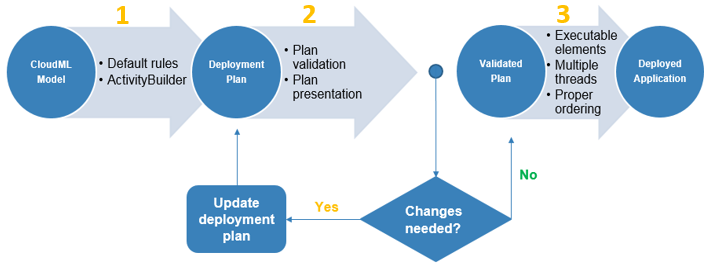
\includegraphics[width=38em]{./Figures/Details}
		\rule{38em}{0.5pt}
	\caption[Approach Details]{Approach details}
	\label{fig:details}
\end{figure}

\noindent 

\begin{figure}[htbp]
	\centering
		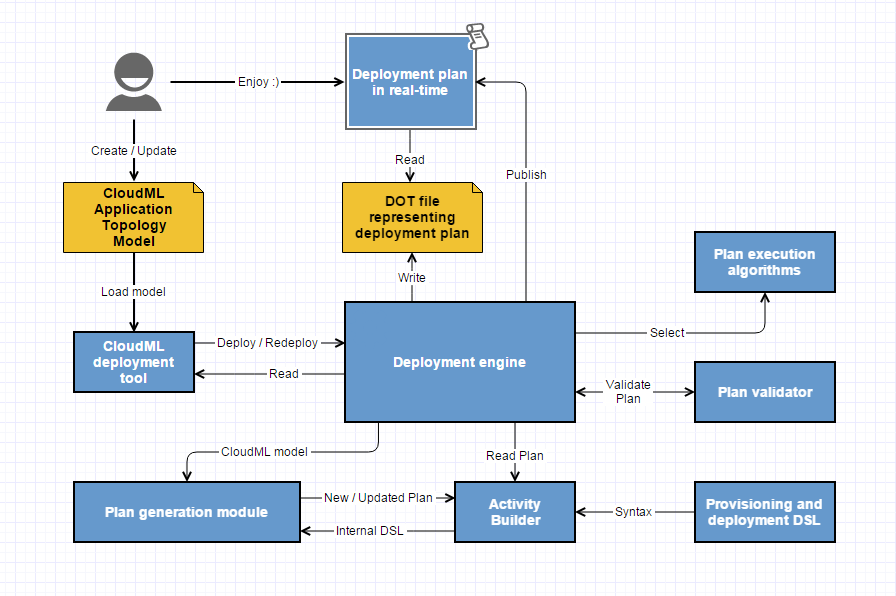
\includegraphics[width=38em]{./Figures/Architecture}
		\rule{38em}{0.5pt}
	\caption[Solution Architecture]{Solution architecture}
	\label{fig:architecture}
\end{figure}

\noindent 

\noindent Figure \ref{fig:architecture} depicts the overall architecture of the deployment system. The core element here is the deployment engine which orchestrates all other components. Referring to the deployment phases defined in the Figure \ref{fig:details}, during the first phase, the Deployment engine submits CloudML model to the Plan generation module. After that, according to the default rules and using the Internal DSL from the Activity Builder, the deployment plan is generated by the Plan generation module and saved in the Activity Builder. During the second deployment phase, the Deployment engine validates the plan through the Plan validator module and generates a DOT file (see Section \ref{subsec:presentation}) which can be used to visualize the deployment plan. Finally, during the third phase the Deployment engine executes the Deployment plan with selected algorithm and the execution process is displayed in real-time to the user.

%----------------------------------------------------------------------------------------

\subsection{Transformation of the Deployment Topology into Deployment Plan} 

\noindent The next step is to discuss each transformation in more details. First, we explain the transformation from the CloudML model to the Deployment Plan. Transformation in this case is based on a set of the default provisioning and deployment rules and on the generation of the Activity Diagram (deployment plan) nodes and edges with a help of our internal DSL, as discussed before. There are four default rules that are executed 

\begin{center}
	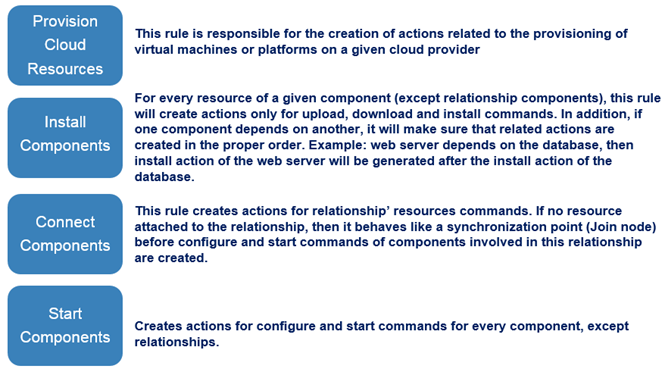
\includegraphics[width=38em]{./Figures/Rules}
	\begin{lstlisting}[mathescape,caption={Default rules of the CloudML deployment engine},label={lst:12}]
	\end{lstlisting}
\end{center}  

\noindent sequentially and they are explained on Listing \ref{lst:12}. These rules execute commands associated to CloudML components. In CloudML each component may have a resource attached to it and such resource may contain several commands like download, install, configure, start. Components may be databases, web servers, relationships.

\noindent During the execution of each rule, ActivityBuilder is used to create relevant components of the deployment plan. This is how the transformation from the CloudML model to the Deployment plan is done. Another interesting details is to understand how created actions are related to the real API calls to deploy the application. We can explain this with an example. For instance, let us take the declaration of the install command method from the CloudML:

\begin{center}
	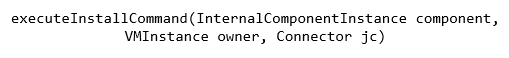
\includegraphics[width=38em]{./Figures/Install}
	\begin{lstlisting}[mathescape,caption={Install command declaration},label={lst:13}]
	\end{lstlisting}
\end{center}

\noindent We can not call this command during the creation of the deployment plan, but we have to know that exactly this command with such parameters must be called in the future. This can be accomplished by creating an Action with input objects that correspond to the input parameters of the executeInstallCommand and by setting the name of the action to ``executeInstallCommand''. This name can be used later to create a call to an actual method at run-time with the help of the Java reflection API\footnote{ The Java Reflection API, $  $https://docs.oracle.com/javase/tutorial/reflect/}. Assuming we have our input objects, we can create an action with multiple inputs like this:

\begin{center}
	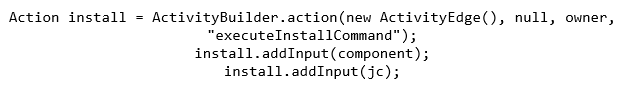
\includegraphics[width=38em]{./Figures/Inputs}
	\begin{lstlisting}[mathescape,caption={Passing data to actions},label={lst:14}]
	\end{lstlisting}
\end{center}

\noindent Apart from this detail, on Figures \ref{fig:provision}-\ref{fig:start_rule} we depict small algorithms to create a deployment plan in the context of the default deployment rules of the CloudML. During the execution of the Provision Cloud Resources rule (Figure \ref{fig:provision}) we have to create corresponding actions and nodes, but creation depends on the number of VMs. If we have several of them, then Fork node must be create and a Join node to gather data flows from all provisioning actions. Otherwise, if there was only one VM we could connect it directly to the Object node which stores IP addresses.

\noindent 

\begin{figure}[htbp]
	\centering
		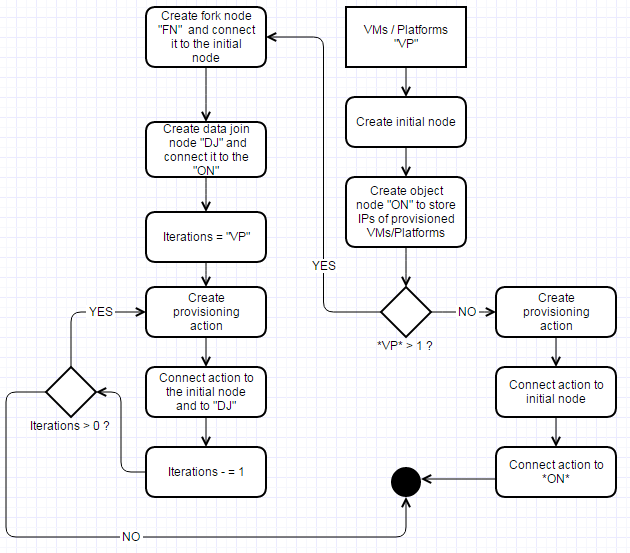
\includegraphics[width=38em]{./Figures/Provision_cloud_resources}
		\rule{38em}{0.5pt}
	\caption[Provisioning Rule]{Creation of the deployment plan during the execution of the Provision Cloud Resources rule}
	\label{fig:provision}
\end{figure}

\noindent 


\noindent 

\begin{figure}[htbp]
	\centering
		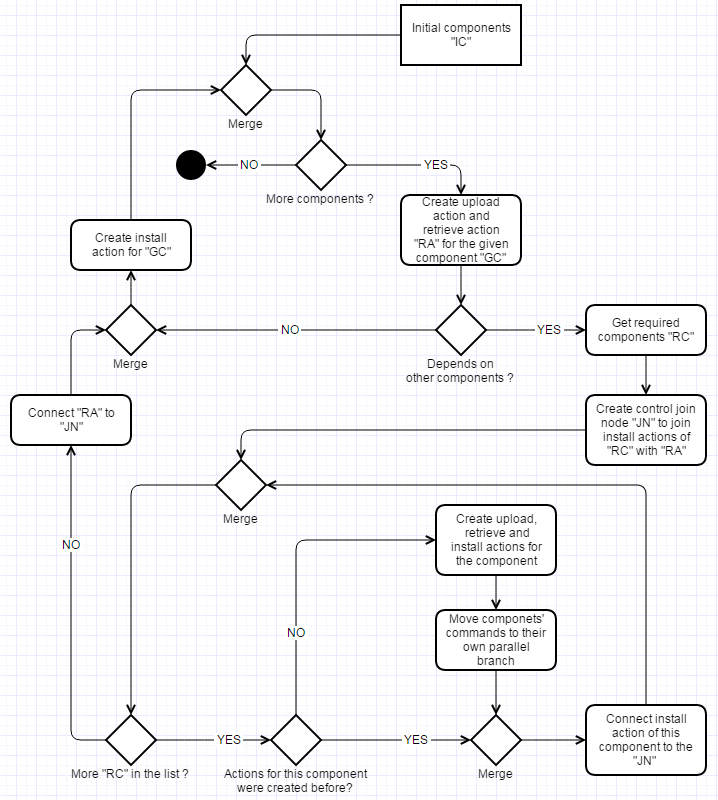
\includegraphics[width=38em]{./Figures/Install_components}
		\rule{38em}{0.5pt}
	\caption[Installation Rule]{Creation of the deployment plan during the execution of the Install Components rule}
	\label{fig:install_rule}
\end{figure}

\noindent

\noindent On Figure \ref{fig:install_rule} an algorithm to create components' install actions is showed. Imagine a servlet component which relies on the Tomcat server, which needs an SQL database to function properly. Assume SQL component was first in the list of components, then all installation actions for the SQL would be created. Then, second component is our servlet. The algorithm would detect that Tomcat must be installed, but before that -- SQL. Because SQL actions were already created, only actions for Tomcat will be generated, and only after that -- actions for the servlet component. 

\noindent 

\begin{figure}[htbp]
	\centering
		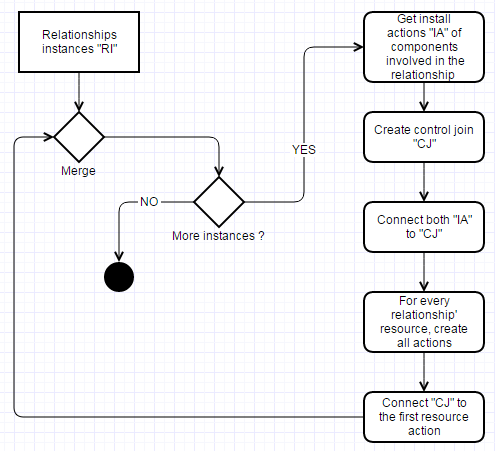
\includegraphics[width=38em]{./Figures/Connect_components}
		\rule{38em}{0.5pt}
	\caption[Connection Rule]{Creation of the deployment plan during the execution of the Connect Components rule}
	\label{fig:connect_rule}
\end{figure}

\noindent 

\noindent Figure \ref{fig:connect_rule} shows a simple algorithm which joins install actions of both components involved in the relationship. After that it creates actions that handle components' resources. If both involved components have attached resource, then additional Fork and Join nodes must be created to allow parallel execution of the resources actions.

\noindent 

\noindent Finally, the algorithm on Figure \ref{fig:start_rule} depicts the creation of configure and start actions. General rule is to connect the install action of the component to its configure action, and then configure action to the start action. In case a given component depends on another one, we create a Join node that synchronizes configure action of the current component with start action of the required component. After that Join node is connected to the start action. Finally, when all actions of all components are created, we join all deployment plan branches (usually each branch represents installation and configuration of one component) and create a Final node. That is when the transformation from the deployment topology to the deployment plan is completely finished. 

\noindent 

\begin{figure}[htbp]
	\centering
		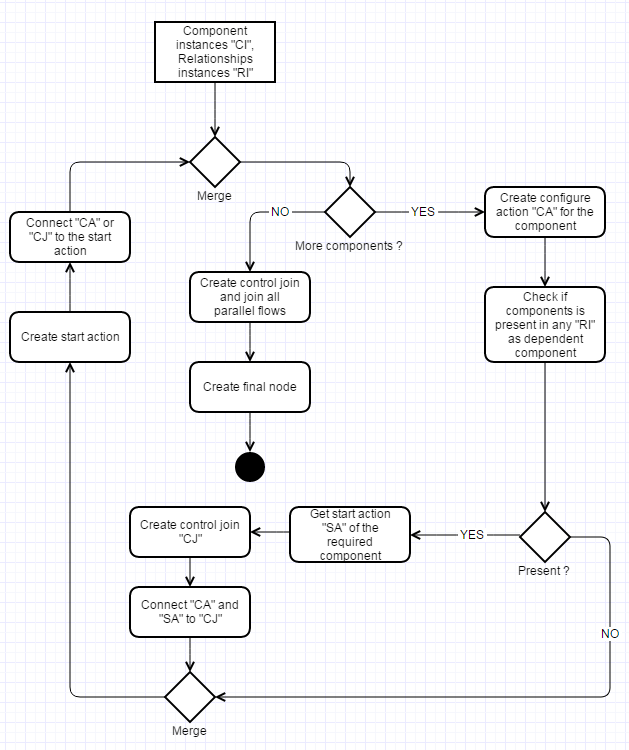
\includegraphics[width=38em]{./Figures/Start_components}
		\rule{38em}{0.5pt}
	\caption[Starting Rule]{Creation of the deployment plan during the execution of the Start Components rule}
	\label{fig:start_rule}
\end{figure}

%----------------------------------------------------------------------------------------

\subsection{Deployment Plan Validation and Presentation} 
\label{subsec:presentation}

\noindent The second step in our approach is the validation and presentation of the deployment plan. Validation is done according to the rules we defined before. After the validation is done, it is important to present the plan to the user. Ideally there would be some running web service that consumes our plan, displays it to the user and allows interactive manipulations. It would require a lot of time and work, so in the current implementation we went for rather a simplistic approach where DOT\footnote{ DOT language, $  $http://www.graphviz.org/pdf/dotguide.pdf} file is generated and presented to the user in the web page. It can also be represented with a help of many free online tools such as GraphvizFiddle\footnote{ GraphvizzFiddle tool, $  $http://stamm-wilbrandt.de/GraphvizFiddle/}. DOT language allows drawing directed graphs as hierarchies, so it nicely fits our needs as deployment process is a set of actions executed one after another. The syntax is quite simple and Listing \ref{lst:15} depicts a fragment of the DOT file and its representation on Figure \ref{fig:dot_image}:

\begin{center}
	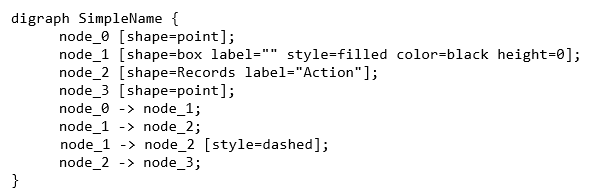
\includegraphics[width=38em]{./Figures/Dot}
	\begin{lstlisting}[mathescape,caption={Fragment of the DOT file},label={lst:15}]
	\end{lstlisting}
\end{center}

\begin{figure}[htbp]
	\centering
		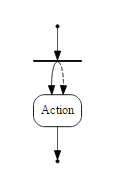
\includegraphics{./Figures/dot_image}
		\rule{38em}{0.5pt}
	\caption[DOT Image]{An image generated from the DOT file}
	\label{fig:dot_image}
\end{figure}

\noindent 

\noindent The whole syntax consists from nodes (node\_0 for instance) which can have different properties and edges that connect nodes (node\_0 -$>$ node\_1) and also may have some properties. To show something more complex, below are two deployment plans: first generated for the storm example and the second - for another application with a bit more complex CloudML model in terms of dependencies between components.  

\noindent 

\noindent On the Figure \ref{fig:storm_deployment}, which shows the storm deployment plan, a reader can observe a few consequent join nodes without any actions between them - this happens because every component is expected to have all set of commands by default: upload, download, install, configure, start. Moreover, if some component does not have configure and start commands for instance - such ``gap'' will be created. This is not an issue as it does not affect execution anyhow, and it may be improved in the future to have a cleaner representation of the plan. One more question that may arise - how can we know the IP of which machine is passed to ``configure:connection\_NameOfCommand'' commands as it is not written explicitly on the data edge? Relationships are components that involve cooperation between two components. The component where a specific command will be executed can retrieve its own IP, so we only need to get an IP of the ``partner''. Take a look at ``configure:connectionRetrieve nimbus-i'' action: ``nimbus-i'' part of the name indicates that this command will be executed on the ``nimbus (Maksym)'' virtual machine. So we need to get IP of the other component involved in the relationship. Before ``configure:connectionRetrieve nimbus-i'' action there is a join node that connect install commands of the zookeeper and nimbus components, so our ``partner'' here is zookeeper component. This means that data edges that lead to ``configure:connectionRetrieve nimbus-i'' and ``configure:connection - Configure nimbus-i'' are passing IP address of the ``zookeeper (Maksym)'' virtual machine.

\noindent 

\begin{figure}[htbp]
	\centering
		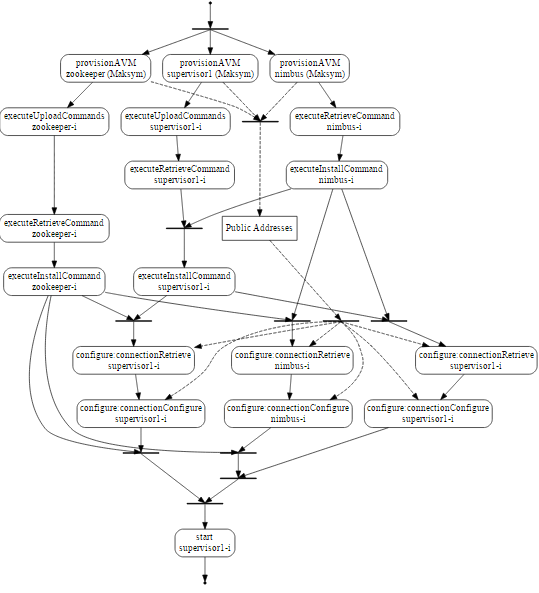
\includegraphics[width=38em]{./Figures/Storm_deployment_plan}
		\rule{38em}{0.5pt}
	\caption[Storm Deployment Plan]{Storm deployment plan}
	\label{fig:storm_deployment}
\end{figure}

\noindent 

\noindent The previous example was simple in a sense that each virtual machine had only one component installed on it and then we had six commands to configure relationships between each component. The deployment plan for another application that we tested is shown on Figure \ref{fig:hierarchy_plan}. It differs from the previous example in the number of components per virtual machine and dependencies between them. In this application we could talk about horizontal and vertical dependencies between components. By horizontal dependency we mean a connection between two independent components - like in the figure below sensApp1 component requires connection to the mongoDB1 component (it is a database). By vertical dependency we mean a situation when one component relies on the other, it just can not be installed without the first one being available - in our case sensApp1 (it is a servlet) needs jettySC1 component (servlet engine) to be installed, the same as sensAppAdmin1 component needs jettySC2 component.

\noindent 

\begin{figure}[htbp]
	\centering
		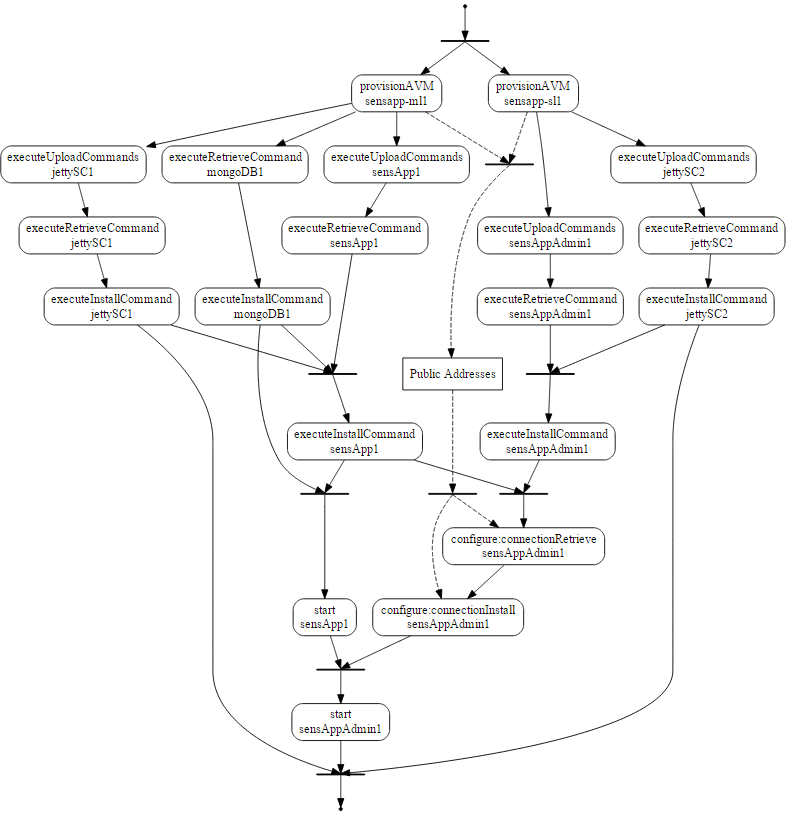
\includegraphics[width=38em]{./Figures/Sensapp_noSaas}
		\rule{38em}{0.5pt}
	\caption[Multi-level Hierarchy Plan]{Deployment plan of the application with multi-level dependency hierarchy}
	\label{fig:hierarchy_plan}
\end{figure}

\noindent 

\noindent To sum up, both examples presented before expose enough details about the deployment and provisioning commands and their ordering, so that the application developer can make a proper decision if the deployment process will be successful or some more adjustments to the plan are needed. In case the application owner decides to adjust the generated plan, he can do that with the help of the internal DSL which was described previously, so we will not go into details how to do it again.

%----------------------------------------------------------------------------------------

\subsection{Deployment Plan Enactment}

\noindent The next phase is the actual deployment of the application. Having the deployment plan generated and validated, the deployment engine has to traverse the graph in the proper order (taking into account parallelization and synchronization points) and execute each task. The execution of every task was covered before -- it is done with the help of Java Reflection API. As for parallelization and synchronization of separate graph branches, we use Java Fork/Join Framework\footnote{ Java Fork/Join framework: https://docs.oracle.com/javase/tutorial/essential/concurrency/forkjoin.html} which allows to start multiple threads asynchronously and join them later. 

\noindent The most difficult part of the plan execution is to actually make sure that every node and edge is visited and visited in a proper order. During the development of the prototype we actually came up with two approaches to traverse the graph. The first approach was inspired by the parallel breadth-first search algorithms which are often used to traverse graphs \cite{akeila2010object}. The idea here is to mark every node and edge with a number (``level'') and then execute nodes and edges of the same level in parallel (using the Fork/Join framework in our case). The leveling of node and edges is depicted on Figure \ref{fig:levels}.

\noindent 

\begin{figure}[htbp]
	\centering
		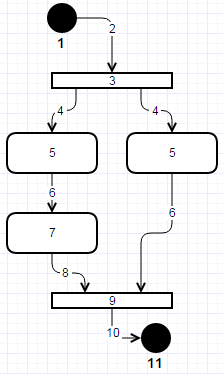
\includegraphics[height=18em]{./Figures/Parallel}
		\rule{38em}{0.5pt}
	\caption[Parallel Algorithm]{Assigning levels to the nodes and edges of the graph}
	\label{fig:levels}
\end{figure}

\noindent 

\noindent It is important to mention that levels do not represent the shortest distance from the source node, but rather the longest distance due to synchronization points. The limitation of such approach is that we achieve parallelism, but not concurrency -- distinct graph branches are not independent. In other words, executing tasks by levels is the same as having Fork and Join nodes for every set of parallel tasks . Thus, this approach is definitely faster than sequential execution of tasks, but not optimal.

\noindent To overcome this limitation, we developed another approach where each parallel branch can be executed in total independence from other branches as shown on Figure \ref{fig:concurrent}, thus achieving concurrency. In this approach, the deployment engine creates a number of threads whenever the it enters Fork node (explicit fork) or Action node with multiple outgoing edges (implicit fork), and joins multiple threads whenever it reaches Join node (explicit join) or Action node with multiple incoming edges (implicit join). Examples of the implicit fork and join are shown on Figure \ref{fig:implicit}. We do not cover many details of both approaches not to overload the reader with technical nuances, the source code is available for curious readers. 

\noindent 

\begin{figure}[htbp]
	\centering
		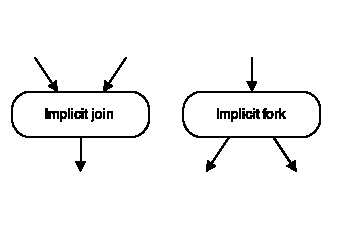
\includegraphics{./Figures/Implicit}
		\rule{38em}{0.5pt}
	\caption[Implicit Fork and Join]{Examples of the implicit fork and join}
	\label{fig:implicit}
\end{figure}

\noindent 

\begin{figure}[htbp]
	\centering
		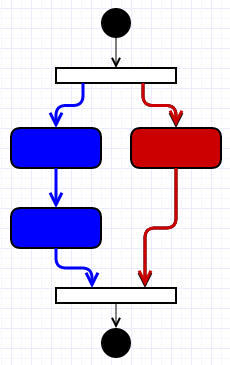
\includegraphics[height=18em]{./Figures/Concurrent}
		\rule{38em}{0.5pt}
	\caption[Concurrent Algorithm]{Execution concurrency: blue and red branches are independent threads}
	\label{fig:concurrent}
\end{figure}

\noindent

\noindent At the moment of writing, the second approach is operational but not yet fully stable - once in a while a deadlock may occur (5-10\% of the time). This will be fixed by the end of the internship. Nevertheless, it proved to be very useful during the development, testing and for the deployment of small applications. In the future, both approaches may be combined to have a robust concurrent deployment algorithm.

\noindent Another important development which resulted from the usage of the models@run-time pattern and from the graphical representation of the deployment plan is that our deployment plan is also a model@run-time. Each node and edge may be in one of the three states: Inactive, Active and Done. Before the graph traversal starts, all nodes and edges are in the state Inactive. Whenever the deployment engine enters some node or edge, it changes the state of that node or edge to Active and then to Done, when it exits that node or edge. All these state changes are reflected in the DOT file. To show this behavior in real time, we created a web page that displays the deployment process in real time. An example of the deployment process is shown on Figure \ref{fig:realtime}.

\noindent Last, but not least, is the description of the continuous deployment process. As we stated before, CloudML has a diff engine which calculates the differences between the old and a new application topology models. With regard to deployment plans, we could follow the same approach -- generate a deployment plan for the new model and then calculate the differences between the old and new plans to create an adaptation plan. Instead, we follow more efficient approach: the plan generation module takes as input new components of the application topology plan and removed components in comparison with the old application topology model. After that, based on the input components, an adaptation plan is generated. By following this approach we eliminate the need to create another diff engine just for the deployment plans by reusing existing algorithms for the plan generation. While generating an adaptation plan, the old deployment plan stays in memory to access important information from the previous deployments, such as IPs of provisioned virtual machines. Thus, the generation of the adaptation plan is based not only on the input components described above, but also on already executed actions. For instance, during the creation of the relationship actions, if require component was installed and started before, it will not be shown again in the adaptation plan. An example of the adaptation plan is shown on Figure \ref{fig:adaptation} -- it is generated after changing the application topology model of the storm cluster from having one supervisor node to two.

\noindent 

\begin{figure}[htbp]
	\centering
		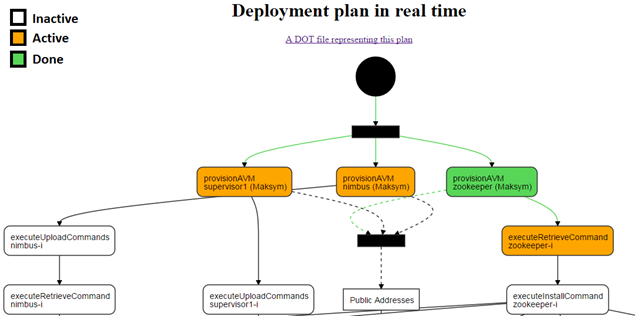
\includegraphics[width=38em]{./Figures/Realtime}
		\rule{38em}{0.5pt}
	\caption[Real-time Deployment]{Deployment process in real time}
	\label{fig:realtime}
\end{figure}

\begin{figure}[htbp]
	\centering
		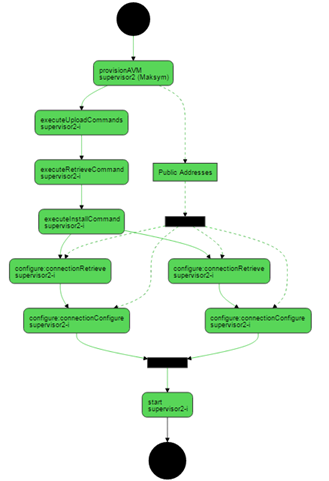
\includegraphics{./Figures/Adaptation}
		\rule{38em}{0.5pt}
	\caption[Adaptation Plan]{Adaptation plan of the storm cluster}
	\label{fig:adaptation}
\end{figure}


\noindent To conclude, the whole process of the deployment plan generation and execution is very complex. While we present a prototype, still a lot has to be done to generate proper plans from different application topologies, to generate proper adaptation plans in various continuous deployment scenarios and to have stable, yet fast, deployment execution algorithms. 




% Chapter 1

\chapter{Evaluation} % Main chapter title

\label{Chapter4} % For referencing the chapter elsewhere, use \ref{Chapter1} 

\lhead{Chapter 4. \emph{Evaluation}} % This is for the header on each page - perhaps a shortened title

%----------------------------------------------------------------------------------------
\noindent In this chapter we validate and evaluate our designs. Validation is important to prove that our approach works and evaluation -- to analyze how good it performs.

\section{Approach Validation}

\noindent First, to validate the whole application provisioning and deployment approach, we have to refer back to the requirements defined in Section 2. The two requirements that were not satisfied by the CloudMF approach were: (i) a domain-specific workflow definition language to describe deployment plans and (ii) possibility to refine the default deployment plan. With the creation of the deployment and provisioning DSL and an internal DSL to manipulate the deployment plans, we can safely state that both requirements are satisfied now. 

\noindent Next, to actually validate our approach, several applications were deployed:

\begin{enumerate}
\item  Storm cluster, which was described in the motivating example and consists of nimbus node, zookeeper node and supervisor node.

\item  SensApp \footnote{ SensApp 1 VM, https://github.com/SINTEF-9012/cloudml/blob/master/docs/samples/sensapp-v2.json}(1 VM): is an open-source application for storing and exploiting data sets collected from different sensors. In this application topology model all SensApp components are installed on one virtual machine.

\item  SensApp\footnote{ SensApp 2 VMs, https://github.com/SINTEF-9012/cloudml/blob/master/docs/samples/sensappAdmin-v2.json} (2 VMs): SensApp admin component is hosted on another virtual machine. The deployment plan for a SensApp with two virtual machines was depicted on Figure 15. 
\end{enumerate}

\noindent All deployments were performed on a Windows 7, 64-bit OS with Intel Core i7-3520M processor and 8 GB of RAM, with such resource consuming applications as Google Chrome web browser and Intellij Idea IDE running at the same time. 

\noindent The Storm cluster application was chosen for experiments because it is a good example of a distributed application with a master-slave architecture. While each component of a Storm cluster is hosted on a separate VM, every VM has only one component installed. That is why SensApp application was taken for the second experiment -- in SensApp the software stack is more complex and there are more dependencies between different components. Finally, SensApp with two VMs was chosen to show how bursting out scenarios could be achieved with our approach. For instance, SensApp admin component could have a policy that it needs a certain amount of CPU to be available for proper operation. When the policy threshold would be reached, a reasoning engine could update the application topology model and redeploy SensApp application. After the redeployment, SensApp application would be running on one VM, and SensApp admin -- on another. Because CloudMF does not support policies yet, we simply updated the model by hand and executed redeployment.

%----------------------------------------------------------------------------------------
\section{Approach Evaluation}

\noindent In addition to the aforementioned deployments, we evaluated several deployment execution approaches in terms of the response time: sequential, parallel and concurrent execution of tasks. The results of our experiments are shown in Table \ref{tab:3}. On Figure \ref{fig:algorithms} we can clearly see that the concurrent algorithm is the fastest one in all three cases. In addition, considering the result depicted in the Figure \ref{fig:sensapp_times}, when the number of the application's components increases (SensApp with 2 VMs with respect to the SensApp with 1 VM), the execution time of the sequential approach obviously increases too, whilst when using the parallel approach it decreases. 

\begin{center}	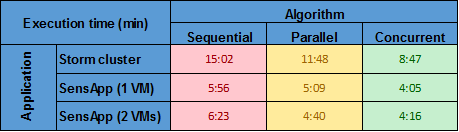
\includegraphics{./Figures/deployment_times}
	\begin{table}[htbp]
    \caption{Application Deployment Times}
    \label{tab:3}
	\end{table}
\end{center} 

\noindent 

\begin{figure}[htbp]
	\centering	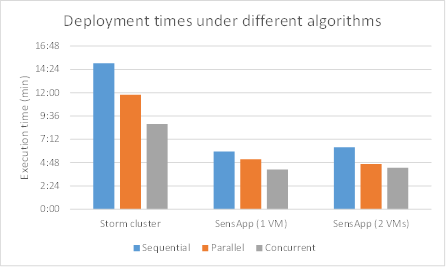
\includegraphics{./Figures/deployment_comparison}
		\rule{38em}{0.5pt}
	\caption[Comparison of Algorithms]{Comparison of deployment algorithms}
	\label{fig:algorithms}
\end{figure}

\noindent 

\begin{figure}[htbp]
	\centering	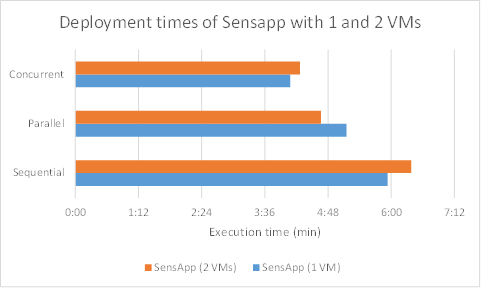
\includegraphics{./Figures/deployment_sensapp}
		\rule{38em}{0.5pt}
	\caption[Comparison of SensApp Execution Times]{Comparison of deployment algorithms when number of application components is growing}
	\label{fig:sensapp_times}
\end{figure}

\noindent 

\begin{figure}[htbp]
	\centering	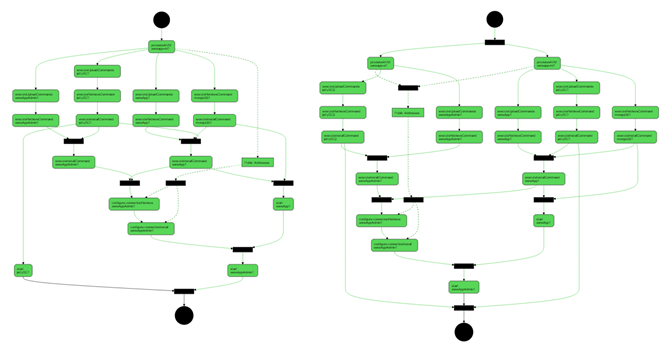
\includegraphics[width=38em]{./Figures/two_vms}
		\rule{38em}{0.5pt}
	\caption[SensApp Deployment Plans]{Deployment plans of the SensApp with 1 VM (left) and 2 VMs (right)}
	\label{fig:sensapp_plans}
\end{figure}

\noindent The reason for that is that bigger number of components, and in particular VMs, allowed the application to utilize parallel threads more efficiently, so the overall deployment time decreased. This can be observed from the Figure \ref{fig:sensapp_plans} where the number of tasks on the deployment plan at the right side of the figure is bigger, but at the same time it has more parallel branches.

\noindent One would expect the same behavior for the concurrent algorithm. Instead, the deployment time under concurrent execution slightly increased. A possible reason for that could be in the structure of the deployment plan. If the plan is relatively symmetric, it does not matter much if one branch can be executed faster than another because they have similar number of tasks (assuming those tasks have similar execution times). In such cases parallel algorithms could probably achieve maximum performance. In scenarios where the plan structure is unbalanced, the number of tasks in every branch differs significantly or there are many forks and joins, independent execution of tasks becomes more important, so concurrent algorithms shall be favored. These are just assumptions, to give a definite answer, a bigger number of experiments with different application topology structures shall be conducted. Moreover, it is out of scope of this work to evaluate efficiency of graph traversal algorithms.

\noindent Another part of evaluation is related to the continuous deployment of cloud applications. We will refer to previous examples: SensApp application with one and two virtual machines. We already know the execution time of the SensApp deployment with two VMs, so the next step is to perform an adaptation: transition from the SensApp application with one VM to SensApp with two VMs. Figure \ref{fig:sensapp_adaptation} shows generated deployment plans in the case of full redeployment (left) and using the CloudML diff engine (right). The execution times and speed-up factors (the ratio between full redeployment and the diff approach) are shown in Table \ref{tab:4}. It may seem strange that execution times for the diff approach are the same under different algorithms, but it can be easily explained if we take a look at the deployment plan in the right part of Figure \ref{fig:sensapp_adaptation}. Two of the most time consuming tasks (installation of the Jetty server and SensApp admin component) has to be executed one after another, while other tasks are performed almost instantaneously. Consequently, the speed-up factor is the biggest for the sequential scenario because there is almost no parallelism and the benefits of parallel and concurrent algorithms can not be exploited.

\begin{center}	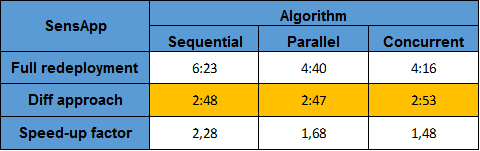
\includegraphics{./Figures/diff}
	\begin{table}[htbp]
    \caption{Evaluation of the Diff Approach}
    \label{tab:4}
	\end{table}
\end{center} 

\begin{figure}[htbp]
	\centering	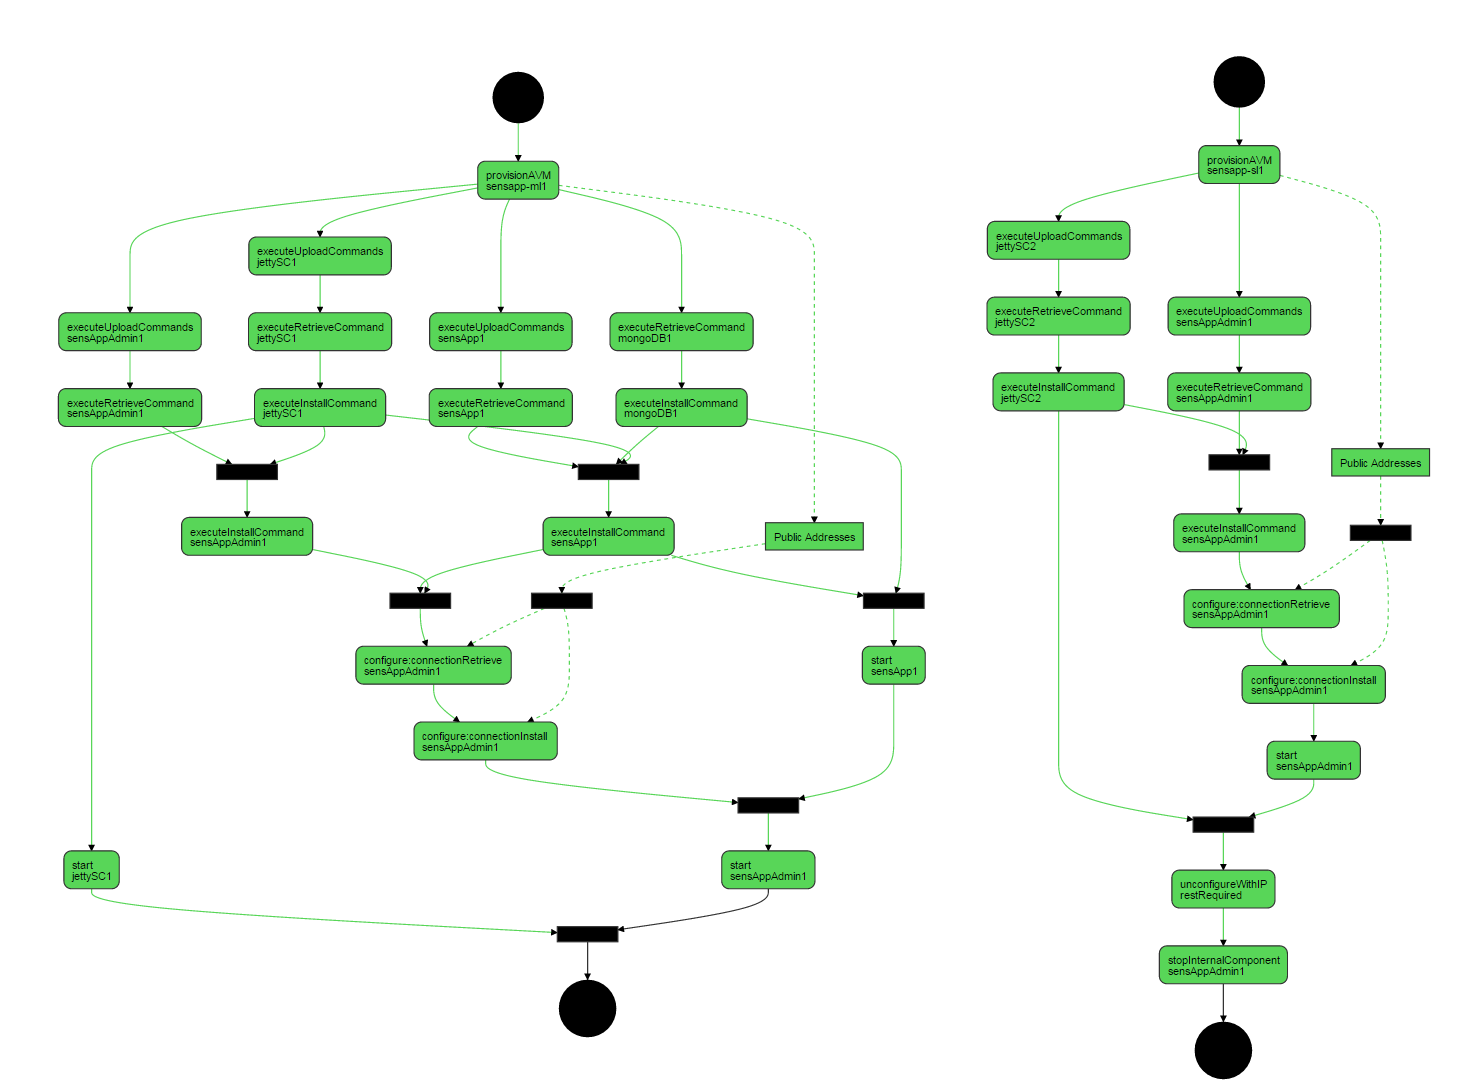
\includegraphics[width=38em]{./Figures/Sensapp_diff}
		\rule{38em}{0.5pt}
	\caption[SensApp Adaptation]{Sensapp (2VMs) deployment plans: full redeployment (left), diff approach (right)}
	\label{fig:sensapp_adaptation}
\end{figure}

\noindent

\noindent The real benefit of the diff approach comes in situations when adaptation plans are quite complex and affect a big part of the application topology. Benefits are achieved in terms of time as shown in the Table \ref{tab:4}, as well as in terms of complexity: the adaptation plan in Figure \ref{fig:sensapp_adaptation} is much simpler than the plan to redeploy the whole application. Simpler adaptation plans are also beneficial in the debugging scenarios -- they are easier to analyze and tune in case something goes wrong. Unfortunately, at the time of writing of this work we did not have application topology models of sufficient complexity to properly highlight the benefits of the diff approach. From the other side, it is intuitive that applying changes only to some part of the application would be faster than redeploying the whole application, especially in the large-scale setups. 

\noindent Finally, we would like to build up on the idea of the combination of parallel and concurrent graph traversal algorithms. If our assumptions, that parallel algorithms are more efficient on symmetric graphs and concurrent -- on asymmetric, are true, then a smart deployment engine could evaluate the deployment plan structure and then apply one or another graph traversal algorithm. A simple idea for evaluation if the graph is symmetric could be to mark graph nodes and edges with levels (as it is currently done in the parallel algorithm) and then compare number of tasks on all levels. If more than half levels have N parallel tasks (N $>$ 2), we could assume the plan is relatively symmetric and apply parallel execution algorithm, otherwise -- concurrent.
 
% Chapter 1

\chapter{Conclusion} % Main chapter title

\label{Chapter5} % For referencing the chapter elsewhere, use \ref{Chapter1} 

\lhead{Chapter 5. \emph{Conclusion}} % This is for the header on each page - perhaps a shortened title

%----------------------------------------------------------------------------------------
\noindent In this work we presented a DSL for the provisioning and deployment of multi-cloud applications which can be used as a library by third parties. In addition, we showed how this DSL was used in the CloudMF framework to combine declarative and imperative deployment approaches. The combination of both approaches allows application developers to deploy applications only by defining the desired final state of the system, while at the same time allowing them to tune the deployment process to their specific needs with help of the internal DSL. Internal DSL could also be used by reasoning engines to automatically update deployment plans according to the defined policies. 

\noindent Moreover, a deployment engine was developed which allows cloud application owners to observe the progress of the deployment process in real-time. The real-time presentation of the deployment process makes it easier to debug applications and gives application operators a clear idea how and when every deployment operation is performed, thus, acting as a decision-support system for the optimization of the deployment process. The deployment engine can deploy applications using parallel or concurrent algorithms to reduce application delivery time, which were also developed as a part of this work. Benefits of such algorithms become essential in the large-scale installations. 

\noindent Finally, we showed how deployment and provisioning DSL can be used in conjunction with model@runtime pattern to perform efficient continuous deployments of cloud applications. Such approach allows for faster redeployments and reduces the complexity of the continuous deployment process by generating adaptation plans which represent updates to the running system, rather than a whole new application state.

\noindent Future work could include the evaluation of the deployment DSL to analyze if it is robust enough to be used in real-world scenarios. In addition, identification of multi-cloud deployment patterns could be interesting to improve the deployment plan generation mechanism. Last, but not least, combination of different deployment execution algorithms could lead to the invention of the next generation deployment engines. 
%\input{./Chapters/Chapter6} 
%\input{./Chapters/Chapter7} 

%----------------------------------------------------------------------------------------
%	THESIS CONTENT - APPENDICES
%----------------------------------------------------------------------------------------


\addtocontents{toc}{\vspace{2em}} % Add a gap in the Contents, for aesthetics

\backmatter

%----------------------------------------------------------------------------------------
%	BIBLIOGRAPHY
%----------------------------------------------------------------------------------------

\label{Bibliography}

\lhead{\emph{Bibliography}} % Change the page header to say "Bibliography"

\bibliographystyle{unsrtnat} % Use the "unsrtnat" BibTeX style for formatting the Bibliography

\bibliography{Bibliography} % The references (bibliography) information are stored in the file named "Bibliography.bib"

\end{document}